\documentclass[5p,twocolumn,number,sort&compress,nopreprintline]{elsarticle}

\usepackage[utf8]{inputenc}
\usepackage[T1]{fontenc}
\usepackage{amsmath,amssymb,amsfonts}
\usepackage{graphicx}
\usepackage{booktabs}
\usepackage{multirow}
\usepackage{tabularx}
\usepackage{placeins}
\usepackage{algorithm}
\usepackage{algpseudocode}
\usepackage{tikz}
\usetikzlibrary{positioning,arrows.meta,shapes,calc,fit,backgrounds}
\usepackage{xcolor}
\usepackage{xurl}
\usepackage{hyperref}
\usepackage{cleveref}

\raggedbottom
\setlength{\emergencystretch}{1.5em}
\setlength{\Urlmuskip}{0mu plus 1mu}


% --- inline code / file names ---
\newcommand{\code}[1]{\texttt{\small #1}}
\newcommand{\figref}[1]{\textbf{\Cref{#1}}}
\newcommand{\tabref}[1]{\textbf{\Cref{#1}}}
\newcommand{\secref}[1]{\textbf{\Cref{#1}}}

% --- figure-source marker (renders as small text, not red) ---
\newcommand{\figsrc}[1]{\par{\footnotesize\textcolor{gray!70!black}{\itshape Source: #1\/}}\par}
% Generated by artifact_pipeline.py; do not edit by hand.
\newcommand{\BenchmarkSizeSet}{\{4,6,8,10,12\}}
\newcommand{\MinQuboCouplings}{6}
\newcommand{\MaxQuboCouplings}{66}
\newcommand{\QAOApOneTwelveRatio}{0.987}
\newcommand{\QAOApOneTwelveHitFraction}{0.33}
\newcommand{\ExactQuboMaxTimeMs}{44}
\newcommand{\QAOApOneMinTime}{0.7}
\newcommand{\QAOApOneMaxTime}{1.7}
\newcommand{\NoisyQaoaMaxTime}{96}
\newcommand{\QraoReportedCompression}{1.00\times}
\newcommand{\RadialInfeasibleSizeSet}{\{4,6,8\}}
\newcommand{\PrefixBaselineMaxTimeMs}{0.200}

% Generated by post_contingency_pipeline.py; do not edit by hand.
\newcommand{\PostContingencyRunCount}{30}
\newcommand{\PostContingencyBestGapMethod}{QAOA p1 noiseless}
\newcommand{\PostContingencyBestMedianGap}{0.500}
\newcommand{\PostContingencyBestMedianGapCILower}{0.250}
\newcommand{\PostContingencyBestMedianGapCIUpper}{0.682}
\newcommand{\PostContingencyBestHitMethod}{QAOA p2 noiseless}
\newcommand{\PostContingencyBestHitFraction}{0.467}
\newcommand{\PostContingencyBestGapRawConnectedRate}{0.000}
\newcommand{\PostContingencyBestGapRawConnectedPercent}{0.0}
\newcommand{\PostContingencyBestGapRawRadialRate}{0.000}
\newcommand{\PostContingencyBestGapRawRadialPercent}{0.0}
\newcommand{\PostContingencyBestGapProjectionRate}{1.000}
\newcommand{\PostContingencyBestGapProjectionPercent}{100.0}
\newcommand{\PostContingencyBestGapSocRate}{0.000}
\newcommand{\PostContingencyBestGapSocPercent}{0.0}
\newcommand{\PostContingencyBestGapAcRate}{1.000}
\newcommand{\PostContingencyBestGapAcPercent}{100.0}
\newcommand{\PostContingencyExactOptimumCount}{1}
\newcommand{\PostContingencySensitivityVariantCount}{11}
\newcommand{\PostContingencySensitivityMinMedianGap}{0.000}
\newcommand{\PostContingencySensitivityMaxMedianGap}{2.167}


% -------------------- metadata --------------------
\bibliographystyle{elsarticle-num}

\begin{document}

\begin{frontmatter}

\title{An Audited ADMM-Inspired Quantum-Classical Workflow for a
Source-Informed Eastern Nepal Transmission Test System}

\author[inst1]{Ujjwal Prasad Dahal}\corref{cor1}\ead{078bel048@student.ioepc.edu.np}

\author[inst1]{Roshan Kumar Sharma}


\cortext[cor1]{Corresponding author.}

\affiliation[inst1]{organization={Department of Electrical Engineering, Institute of Engineering, Purwanchal Campus, Dharan},
                    country={Nepal}}

\begin{abstract}
We present an ADMM-inspired quantum-classical workflow for an
experimental emergency-restoration policy on a 16-bus, 21-branch,
220/132/400 kV Eastern Nepal test system. The system is source-informed
but is not an as-operated utility model: it combines reported assets,
planned circuits, a hypothetical voltage interface, and an estimated
operating point. The classical
$\boldsymbol\alpha$-update
is a second-order-cone (SOC) relaxation of the AC branch-flow (DistFlow)
model; the binary $\boldsymbol z$-update is
a Quantum Approximate Optimization Algorithm (QAOA) running on a
historical topology-coupled Quadratic Unconstrained Binary Optimization
(QUBO) whose cycle and anti-islanding terms are heuristic rather than
hard radiality constraints.
The retained scaling benchmark passed no forced-open branch to either
subproblem; it is therefore a base-case surrogate-QUBO artifact, not
post-contingency evidence. We audit that frozen artifact for
$n\in\BenchmarkSizeSet$, comparing QAOA at $p\in\{1,2\}$, Quantum
Random Access Optimization (QRAO), simulated annealing (SA), and an
exact-QUBO reference solver. The previously reported ``success probability''
is the optimizer-run QUBO-minimum hit fraction
$\widehat h_{\mathrm{run}}^\star$, not a shot-level probability. At
$n=12$, noiseless QAOA at
$p=1$ has a legacy objective ratio of \QAOApOneTwelveRatio{} and an
optimizer-run QUBO-minimum hit fraction of
\QAOApOneTwelveHitFraction{}. More importantly, the topology induced by
current exhaustive enumeration finds disconnected global minimizers at
$n=6,10,12$; this reconstruction is a topology audit, not a claim about
the bitstring returned by the historical solver. The finding demonstrates
that a high surrogate score does not establish engineering validity.
The audited QUBO contains
nonzero cycle terms at every size and anti-islanding terms from $n=8$;
these make the actual QUBO nonuniform, so it is not the easy
cardinality-plus-linear special case. An exhaustive topology audit nevertheless
finds that the forced-closed scaling protocol makes a spanning tree
impossible for $n\in\RadialInfeasibleSizeSet$, and none of the historical
QUBO minimizers at $n=10$ or $12$ is radial. QRAO uses
the same number of qubits as QAOA in the retained runs, while the classical
exact-QUBO solver finishes within \ExactQuboMaxTimeMs{}~ms. Quantitative
ablation and hardware claims are excluded from this frozen result set
because the released repository did not retain their raw evidence.
The continuous model has been corrected for fixed-power-factor shedding,
branch ratings, transformer taps, slack balance, and nonlinear recovery;
the legacy SOC losses are consequently marked stale.

Separately, we execute a predeclared hypothetical N$-1$ outage of
Basantapur--Inaruwa circuit~A (branch~3) with 30 independent runs per
method. QAOA at $p=1$ and $p=2$ share the lowest median QUBO gap,
\PostContingencyBestMedianGap{}, while $p=2$ has the highest
optimizer-run exact-QUBO hit fraction,
\PostContingencyBestHitFraction{}. None of the raw solver outputs is
connected or radial; the declared spanning-tree projection succeeds for
all runs, after which every projected candidate passes the series-only
nonlinear AC validation but none passes the stricter SOC-recovery
certificate. All three exact and all 30 QAOA-based ADMM runs terminate at
the 30-iteration cap rather than the residual tolerances.
No quantum advantage is observed or claimed.
\end{abstract}

\begin{keyword}
Hybrid quantum-classical \sep ADMM \sep QAOA \sep QRAO \sep QUBO \sep
Transmission reconfiguration \sep Optimal transmission switching \sep
Branch-flow SOC \sep Eastern Nepal grid
\end{keyword}

\end{frontmatter}

% =====================================================================
\section{Introduction}
\label{sec:intro}
% =====================================================================

The power grid is, at its operational core, a combinatorial problem:
discrete switching decisions on a continuous physical system. The
\emph{optimal transmission switching} (OTS) problem introduced by
Fisher, O'Neill, and Ferris~\cite{fisher2008ots} made this explicit
for transmission networks, showing that allowing some lines to be
opened under normal operation can reduce dispatch cost, relieve
congestion, and improve security margins. A natural emergency
counterpart is \emph{post-contingency transmission reconfiguration}: a
small set of lines and transformers is forced open (for example, by a fault or
by a maintenance order), and the operator must reconfigure the
\emph{switchable} lines so that the resulting topology is radial under
the emergency-restoration policy studied here, connected, and validated
by stated nonlinear AC checks, with minimal
losses and load-shedding.
This problem is NP-hard in general~\cite{fisher2008ots}, and real
meshed sub-systems have enough switchable branches that a combinatorial
explosion is the rule rather than the exception.

Quantum optimisation has, in the last decade, become a credible tool
to attack combinatorial problems of this kind. The Quantum
Approximate Optimization Algorithm (QAOA) of Farhi, Goldstone, and
Gutmann~\cite{farhi2014qaoa} prepares a depth-$p$ variational state by
alternating a problem Hamiltonian and a mixer. In the minimisation
convention used here, a classical optimiser searches $2p$ parameters
to minimise the expectation of the Ising Hamiltonian obtained from the
QUBO. QAOA is one instance of the broader class of variational quantum
algorithms~\cite{cerezo2021vqa}. QRAO
(Quantum Random Access Optimization) of Fuller \emph{et
al.}~\cite{fuller2024qrao} packs up to $k$ binary variables per qubit
using a $(k,1,p)$-qubit random access code (QRAC), reducing qubit
footprint at the cost of requiring a magic-state rounding step to
recover the binary solution. For both algorithms, the engineering
reality of near-term Noisy Intermediate-Scale Quantum (NISQ) hardware
imposes hard limits on circuit depth, qubit count, and shot budget.
The question of \emph{how} to interface such algorithms with realistic
power-system constraints (AC physics, radiality, connectivity,
operational limits on voltage and current) is the central engineering
question of this paper.

\subsection{The ADMM-QAOA recipe for mixed-integer problems}
A clean way to interface a binary quantum solver with a continuous AC
feasibility problem is consensus ADMM, as in the celebrated
Boyd~\emph{et~al.} formulation~\cite{boyd2011admm}. The
mixed-integer problem is decomposed into a convex continuous
$\boldsymbol\alpha$-subproblem (the generic ADMM ``$x$-update'') and a
combinatorial $\boldsymbol z$-subproblem coupled by a linear consensus
constraint and a dual variable. The quantum solver is used only for the
$\boldsymbol z$-update; the $\boldsymbol\alpha$-update stays
classical and convex. The literature now contains a small but growing
set of demonstrations of this pattern on power-system problems.
Ngo~\emph{et~al.}~\cite{ngo2022evaluate,ngo2024qrao} demonstrated
ADMM-QAOA and ADMM-QRAO on the IEEE 33-bus distribution case for
radial reconfiguration. Ellinas, Chevalier, and
Chatzivasileiadis~\cite{ellinas2024hybrid} proposed a Benders-based
hybrid quantum-classical MILP solver that includes OTS and benchmarked
it on IBM Eagle. Bosmediano~\emph{et~al.}~\cite{bosmediano2026dnr}
studied QAOA reconfiguration of the IEEE 33-bus with AC-feasibility
constraints and renewable generation. Silva~\emph{et~al.}
gave a QUBO formulation for minimum-loss network
reconfiguration~\cite{silva2021qubo}, while Mokhtari~\emph{et~al.}
used classical distributed ADMM with a minimum-weight rooted
arborescence subproblem~\cite{mokhtari2025admm}. Quantum-enhanced ADMM
has also been studied for generation scheduling rather than topology
reconfiguration~\cite{yang2026qreadmm}. Morstyn and
Wang~\cite{morstyn2024joule} and
Morstyn~\cite{morstyn2023annealing} reviewed the role of both gate-based
and annealing-based quantum methods in net-zero power-system
optimisation. Recent preprints further study topology-preserving QAOA
sampling for distribution-grid spanning trees~\cite{hartmann2025spanning}
and structured feasibility repair for power-system
islanding~\cite{jiang2026regrid}. Against this literature, the present contribution is
deliberately bounded: it provides an auditable source-informed regional
test system, an explicit separation between heuristic topology scores
and hard radial references, and a series-only nonlinear AC recovery
check. The July 2026 search record is archived with the review
materials. We claim neither an exhaustive priority result across every
quantum power-system formulation nor operation on an as-operated utility
network.

\subsection{What this paper is, and is not, claiming}
This paper develops the workflow on a source-informed 16-bus Eastern
Nepal topology with estimated nodal loads and injections. The retained benchmark
covers an exact-QUBO reference solver, QAOA, QRAO, and SA. We make the following
contributions:

\begin{enumerate}
\item \textbf{A source-informed regional test system.} We instantiate
the workflow on a 16-bus, 220/132/400 kV Eastern Nepal
(Koshi--Kabeli) test system informed by the NEA Transmission and
Project Management Directorate Year Book for fiscal year
2024/2025~\cite{nea2082yearbook,nea_transmission_map}. The model mixes
reported in-service assets, planned circuits, and a hypothetical
voltage interface. Segment impedances, ratings, taps, the operating
point, and several connections are assumptions, all labelled in the
generated branch-provenance table.

\item \textbf{A topology-coupled QUBO with an exhaustive radiality audit.}
We retain the historical spanning-tree-cardinality, pairwise-cycle,
and anti-islanding objective as an explicitly heuristic surrogate and
separately implement a constraint-exact single-commodity-flow spanning-tree
formulation. The audited union of
off-diagonal pairs grows from \MinQuboCouplings{} at $n=4$ to
\MaxQuboCouplings{} at $n=12$. Component-level accounting corrects the
previous claim that the cycle and anti-islanding matrices were empty,
while exhaustive auditing quantifies their false positives and false
negatives.

\item \textbf{An auditable scaling comparison with classical structure
baselines.} The frozen artifact
retains legacy objective ratios, optimizer-run QUBO-minimum hit fractions, wall times,
QUBO component counts, and the legacy fixed-topology SOC fields that
were actually saved and are now explicitly marked stale. It also contains
an exact sorting/prefix baseline for the cardinality-only special case,
an exhaustive radial enumeration, and a mixed-integer spanning-tree baseline.
In these retained runs QRAO has
$\QraoReportedCompression$ compression, but no causal compression
ablation is claimed without a machine-readable ablation record.

\item \textbf{A reproducible claim pipeline.} One strict JSON file is
the source of truth. The CSV, numerical macros, appendix table, and
benchmark figures are generated from it and recorded by SHA-256 in a
manifest. A separate machine-readable study protocol records the
contingency, archived bit-to-branch ordering, penalties, seeds, stopping rules, and
predeclared statistics for regeneration. Missing ADMM, ablation,
library-baseline, and hardware
evidence is marked as excluded rather than back-filled from prose.
\end{enumerate}

\textbf{What we are not claiming.} We do \emph{not} claim quantum
advantage. The problem sizes are too small (4--12 qubits for the
combinatorial sub-problem), the depth too shallow ($p\le 2$), and the
classical exact-QUBO and SA baselines too strong. The present revision also
does not claim validated hardware performance, because the released
files do not contain the raw evidence needed to audit those jobs. It
also does not claim that the retained numerical
artifact is post-contingency: no branch outage was supplied in those runs.

\subsection{Paper structure}
The remainder of the paper is organised as follows.
Section~\ref{sec:system} introduces the Eastern Nepal sub-system, the
AC branch-flow SOC model, and the optimal reconfiguration problem.
Section~\ref{sec:admm-qaoa} derives the ADMM decomposition, audits the
heuristic QUBO, and gives the flow-based spanning-tree formulation.
Section~\ref{sec:benchmark} defines the
benchmark protocol. Section~\ref{sec:results} reports the audited
scaling results and evidence status, and Section~\ref{sec:discussion} discusses
limitations and methodological lessons. Section~\ref{sec:conclusion}
concludes.

% =====================================================================
\section{System and Problem Formulation}
\label{sec:system}
% =====================================================================

\subsection{The Eastern Nepal sub-system}
\label{sec:system-data}
The implemented case is a 16-bus, 21-branch test system covering the Koshi
Corridor (220 kV) and the Kabeli Corridor (132 kV) in Eastern Nepal,
together with the southern part of the 132 kV Sunsari--Jhapa industrial
cluster. The sub-system is the eastern part of the Integrated Nepal
Power System (INPS) studied in~\cite{bhandari2020inps,shah2023hditl}.
Routes, reported project status, aggregate lengths, and selected
equipment multiplicities are informed by the NEA Transmission and
Project Management Directorate Year Book for fiscal year 2024/2025
(2081/2082)~\cite{nea2082yearbook} and a transmission network
map~\cite{nea_transmission_map}. The model is not an as-operated
network. KC1 circuit~B was planned rather than in service during the
source year, and the Amarpur--Dhungesanghu link was under construction.
Both are included as prospective switchable elements. The latter also
uses a hypothetical 100-MVA 220/132-kV interface because the source
does not report such an interface. Figure~\ref{fig:network} therefore
shows the test system, not a utility single-line record. The slack is
the modeled 400-kV Inaruwa hub. Generation comprises a reported
73-MW Sanima Middle Tamor injection plus assumed 60-MW Tumlingtar and
40-MW Amarpur aggregates.

\begin{figure}[ht]
\centering
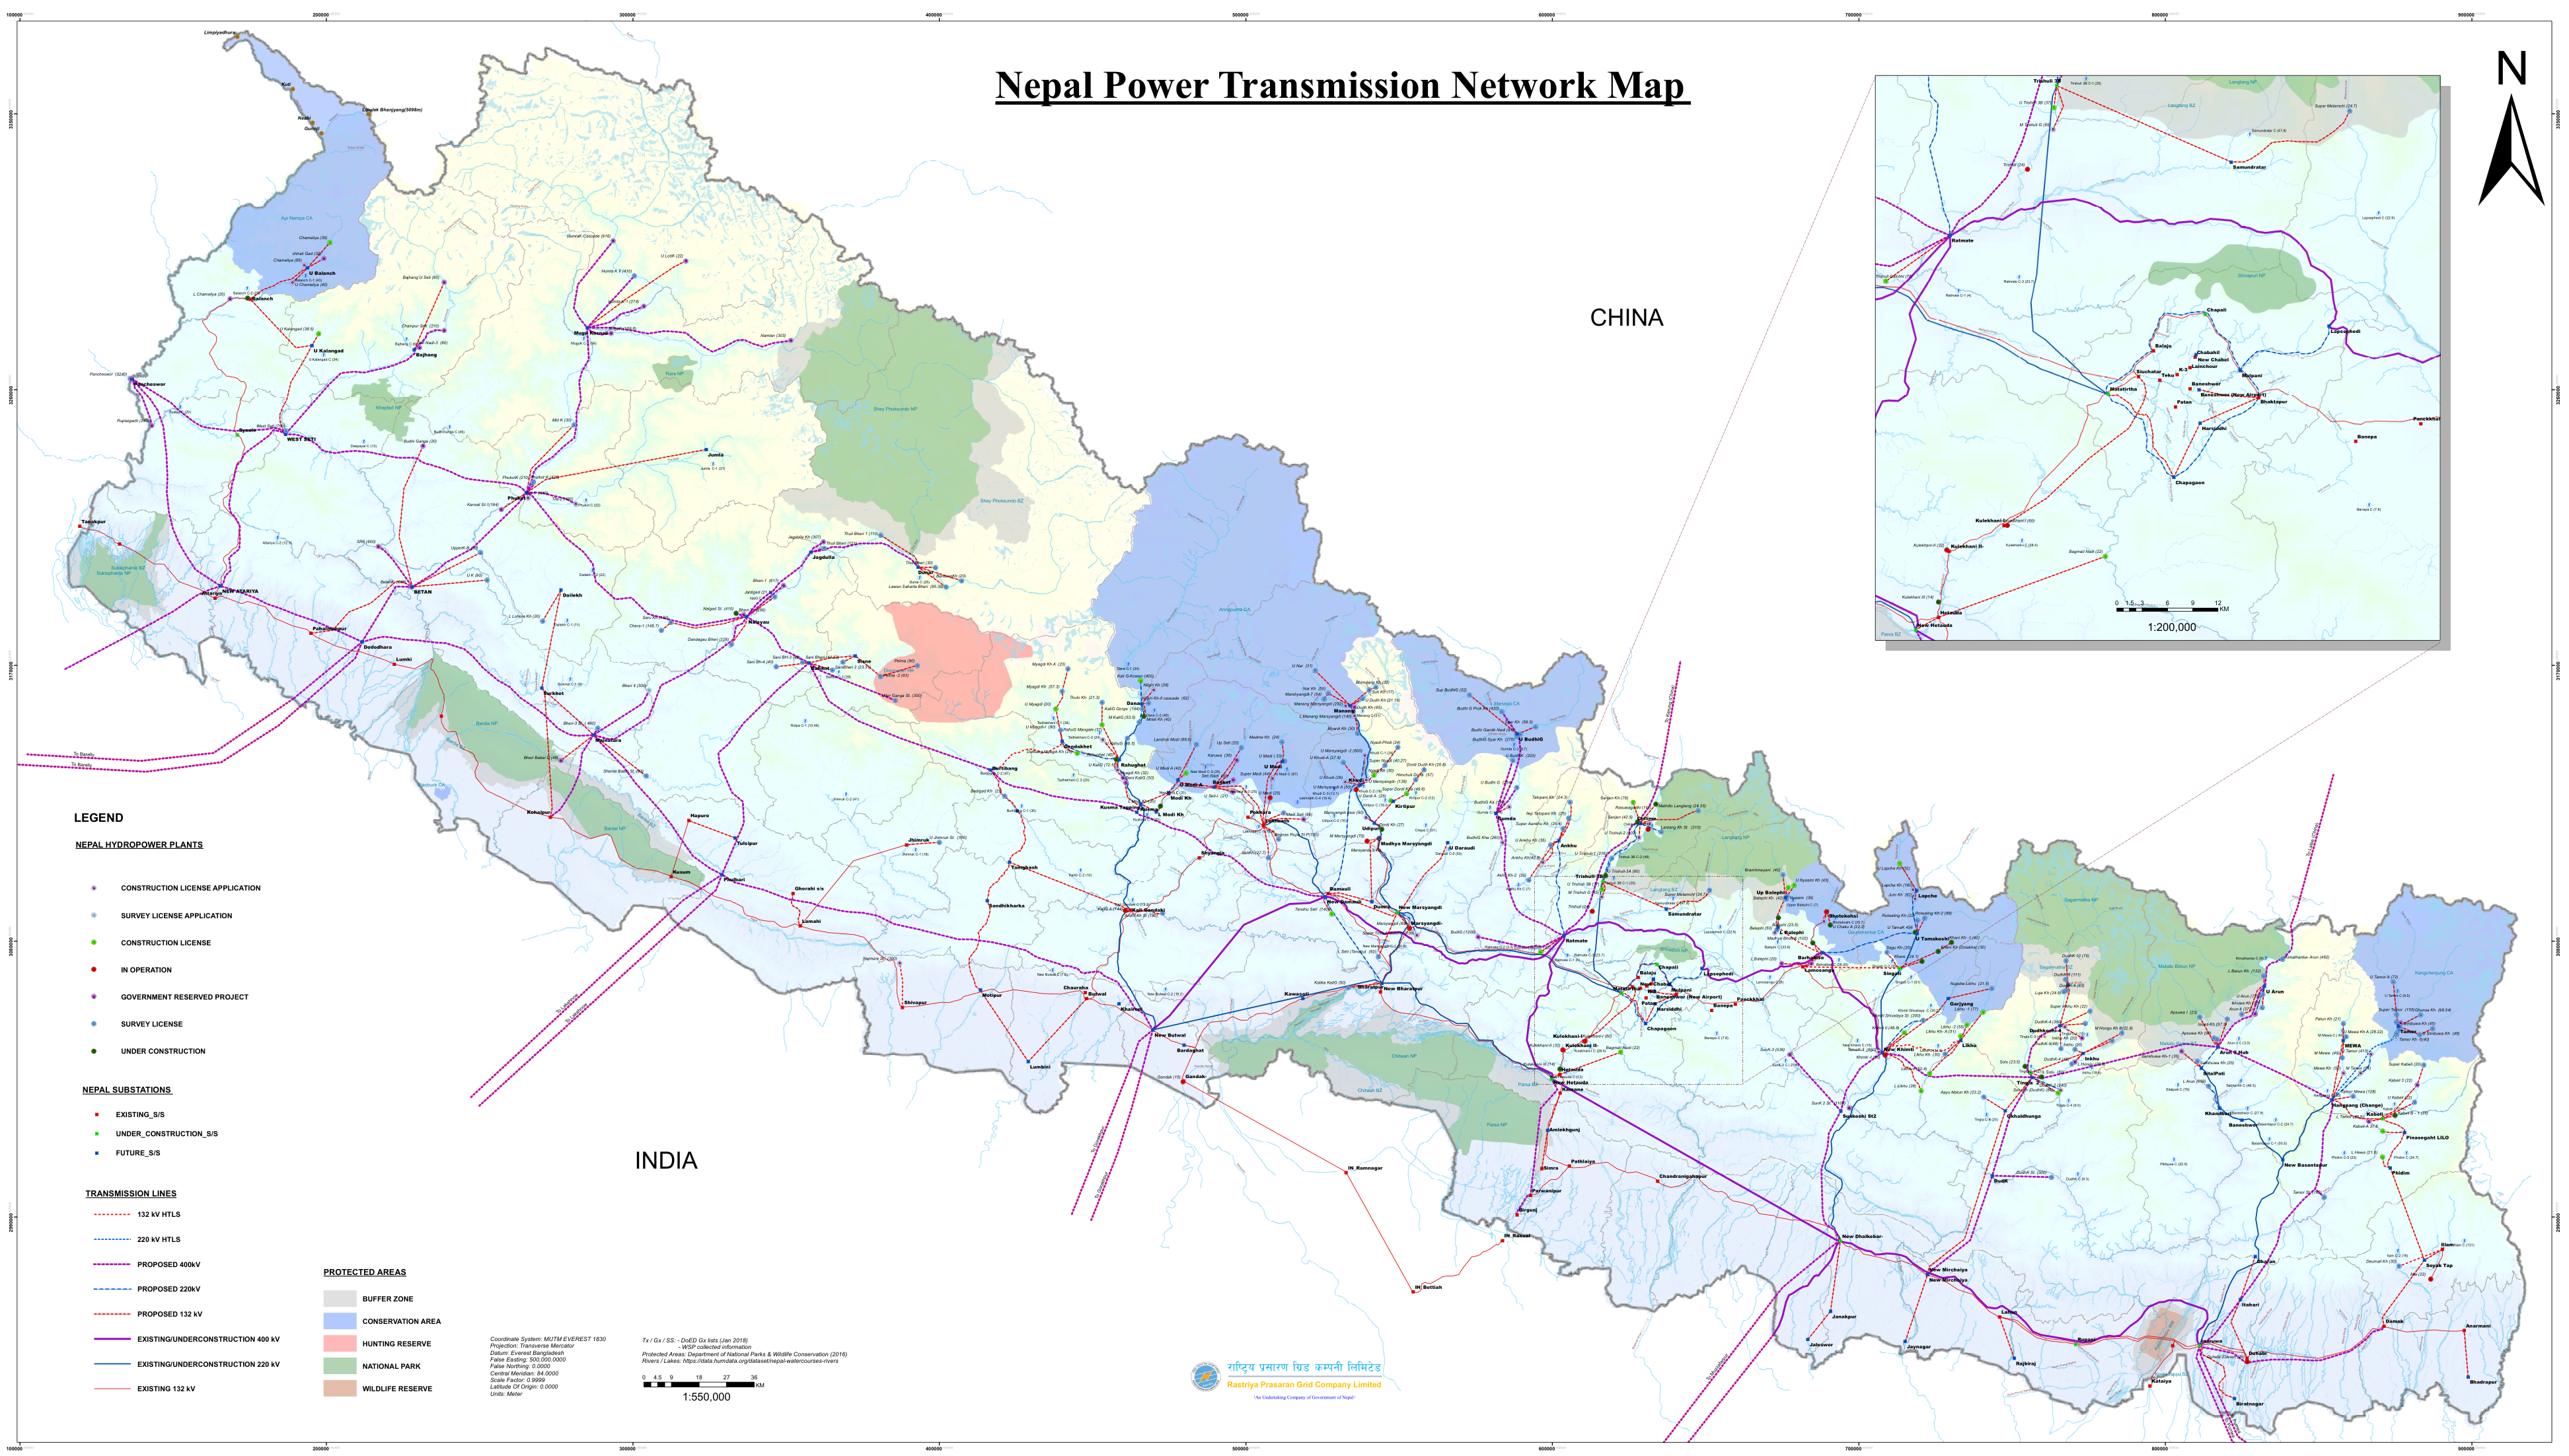
\includegraphics[width=\columnwidth]{figures/nepal_network_map.png}
\caption{One-line diagram of the 16-bus source-informed test system.
The Inaruwa 400-kV bus is the slack; generation injections are marked.
The diagram combines reported, planned, and hypothetical elements as
documented in the branch-provenance table.}
\label{fig:network}
\end{figure}

\paragraph{Network at a glance.}
The 16-bus meshed model has 21 branch records, of which 14 are
switchable. It contains two reported Inaruwa transformer-bank
equivalents and one assumed voltage-interface equivalent.
Table~\ref{tab:network-summary} summarises the modeled quantities.

\begin{table*}[t]
\centering
\caption{Summary of the source-informed Eastern Nepal test system.}
\label{tab:network-summary}
\small
\begin{tabular}{lr}
\toprule
\textbf{Quantity} & \textbf{Value} \\
\midrule
Buses (400 / 220 / 132 kV) & 1 / 5 / 10 \\
Branch records (line / transformer / tie) & 13 / 2 / 6 \\
Switchable branches & 14 \\
Slack bus & Inaruwa 400 kV \\
Generation injection (MW) & 173 (73 reported; 100 assumed) \\
Load (MW) & 485 (assumed) \\
Net demand before losses (MW) & 312 \\
Branch rating range (MVA) & 100--1600 \\
Transformer off-nominal taps (pu) & 1.0 (assumed) \\
Common MVA base & 100 \\
Voltage band (pu) & 0.90 -- 1.10 \\
\bottomrule
\end{tabular}
\end{table*}

% Generated by artifact_pipeline.py; do not edit by hand.
\begin{table*}[t]
\centering
\caption{Branch-level model provenance. Ratings, conductor parameters, several lengths, transformer short-circuit reactances, and operating taps are engineering assumptions unless the source column states otherwise. Parallel transformer units are represented by one equivalent rating and reactance.}
\label{tab:branch-provenance}
\scriptsize
\setlength{\tabcolsep}{2.2pt}
\begin{tabularx}{\textwidth}{rXrrrrrrXX}
\toprule
$k$ & Element & Units & km & $r$ (pu) & $x$ (pu) & MVA & Tap & Status & Source/assumption \\
\midrule
0 & Inaruwa 400/220 & 3 & -- & 0.00000 & 0.01270 & 945 & 1.000 & source-derived + assumed & [D2082] multiplicity/rating; 12\% reactance and tap assumed \\
1 & Inaruwa 220/132 & 2 & -- & 0.00000 & 0.03750 & 320 & 1.000 & source-derived + assumed & [D2082] multiplicity/rating; 12\% reactance and tap assumed \\
2 & Amarpur-Dhungesanghu 132 (tie+xfmr) & 1 & 19.13 & 0.01208 & 0.16392 & 100 & 1.000 & planned topology + assumed interface & [D2082 project 8] planned route/length; all interface, conductor, rating, X\% and tap values assumed \\
3 & Basantapur-Inaruwa ckt-A & 1 & 57 & 0.00177 & 0.02944 & 600 & 1.000 & in-service route + assumed parameters & [D2082 KC1] route and aggregate corridor length; segment length, electrical parameters and rating assumed \\
4 & Basantapur-Inaruwa ckt-B & 1 & 57 & 0.00177 & 0.02944 & 600 & 1.000 & planned circuit + assumed parameters & [D2082 KC5] planned second circuit; segment length, electrical parameters and rating assumed \\
5 & Baneshwar-Basantapur ckt-A & 1 & 30 & 0.00186 & 0.01860 & 600 & 1.000 & in-service route + assumed parameters & [D2082 KC1] route and aggregate corridor length; segment length, electrical parameters and rating assumed \\
6 & Baneshwar-Basantapur ckt-B & 1 & 30 & 0.00186 & 0.01860 & 600 & 1.000 & planned circuit + assumed parameters & [D2082 KC5] planned second circuit; segment length, electrical parameters and rating assumed \\
7 & Tumlingtar-Baneshwar ckt-A & 1 & 20 & 0.00124 & 0.01240 & 600 & 1.000 & in-service route + assumed parameters & [D2082 KC1] route and aggregate corridor length; segment length, electrical parameters and rating assumed \\
8 & Tumlingtar-Baneshwar ckt-B & 1 & 20 & 0.00124 & 0.01240 & 600 & 1.000 & planned circuit + assumed parameters & [D2082 KC5] planned second circuit; segment length, electrical parameters and rating assumed \\
9 & Dhungesanghu-Basantapur ckt-A & 1 & 35 & 0.00217 & 0.02169 & 600 & 1.000 & source-derived + assumed & [D2082 KC3] topology/length; conductor and rating assumed \\
10 & Dhungesanghu-Basantapur ckt-B & 1 & 35 & 0.00217 & 0.02169 & 600 & 1.000 & source-derived + assumed & [D2082 KC3] topology/length; conductor and rating assumed \\
11 & Inaruwa-Dhalkebar 400 & 1 & 84 & 0.00063 & 0.01470 & 1600 & 1.000 & source-derived + assumed & [D2082] topology/approximate length; conductor and rating assumed \\
12 & Inaruwa-Kusaha 132 & 1 & 22 & 0.01389 & 0.05051 & 160 & 1.000 & engineering estimate & [MAP] topology; length, conductor and rating assumed \\
13 & Duhabi-Kusaha 132 & 1 & 28 & 0.01768 & 0.06428 & 160 & 1.000 & source-derived + assumed & [D2082 Package C] topology/length; conductor and rating assumed \\
14 & Duhabi-Itahari 132 & 1 & 15 & 0.00947 & 0.03444 & 160 & 1.000 & engineering estimate & [MAP] topology; length, conductor and rating assumed \\
15 & Itahari-Damak 132 & 1 & 18 & 0.01136 & 0.04132 & 160 & 1.000 & engineering estimate & [MAP] topology; length, conductor and rating assumed \\
16 & Damak-Anarmani 132 & 1 & 45 & 0.02841 & 0.10331 & 160 & 1.000 & engineering estimate & [D2082/MAP] topology; length, conductor and rating assumed \\
17 & Itahari-Dharan 132 & 1 & 16 & 0.01010 & 0.03673 & 160 & 1.000 & engineering estimate & [MAP] topology; length, conductor and rating assumed \\
18 & Amarpur-Phidim 132 & 1 & 58 & 0.03662 & 0.13315 & 160 & 1.000 & engineering estimate & [D2082/MAP] topology; length, conductor and rating assumed \\
19 & Phidim-Godak 132 & 1 & 55 & 0.03472 & 0.12626 & 160 & 1.000 & engineering estimate & [D2082/MAP] topology; length, conductor and rating assumed \\
20 & Godak-Damak 132 & 1 & 60 & 0.03788 & 0.13774 & 160 & 1.000 & engineering estimate & [MAP] topology; length, conductor and rating assumed \\
\bottomrule
\end{tabularx}
\end{table*}


\subsection{Indexing, state, and objective conventions}
\label{sec:notation}
Let $\mathcal B$ be the physical-bus set, $\mathcal E$ the
physical-branch set, $\mathcal E^{\mathrm{sw}}\subseteq\mathcal E$
the switchable branches, and $\mathcal F\subseteq\mathcal E$ the
forced-open contingency set. Buses are indexed by $i,j$, and physical
branches by $k$. Let
$\mathcal D\subseteq\mathcal E^{\mathrm{sw}}\setminus\mathcal F$ be
the switchable branches included in a particular binary experiment,
$n=|\mathcal D|$, and
$\pi:\{0,\ldots,n-1\}\to\mathcal D$ the archived variable-order map.
The mandatory-closed set is
$\mathcal E^{\mathrm{mand}}=\mathcal E\setminus
(\mathcal F\cup\mathcal D)$.
Vector positions are indexed by $\ell,m$; thus $z_\ell$ is the binary
decision for physical branch $\pi(\ell)$. The continuous ADMM copy is
$\boldsymbol\alpha\in[0,1]^n$, the binary ADMM/QUBO copy is
$\boldsymbol z\in\{0,1\}^n$, and a solver-returned or measured bitstring
is denoted $\boldsymbol b\in\{0,1\}^n$. A raw solver output is
$\boldsymbol b^{\rm raw}$; after the explicitly reported spanning-tree
projection it is $\boldsymbol b^{\rm proj}$. These objects use the same
archived order but have different roles. In particular, a projected
bitstring is never relabelled as the solver's raw output.

For $\boldsymbol v\in\{\boldsymbol\alpha,\boldsymbol z,
\boldsymbol b^{\rm raw},\boldsymbol b^{\rm proj}\}$, the physical branch
gate is
\begin{equation}\label{eq:physical-gate-map}
a_k(\boldsymbol v)=
\begin{cases}
0, & k\in\mathcal F,\\
v_\ell, & k=\pi(\ell),\\
1, & k\notin\mathcal F\cup\mathcal D.
\end{cases}
\end{equation}
The last case includes available fixed branches and switchable branches
forced closed by a legacy prefix experiment. Branch impedance is
$\zeta_k=r_k+\mathrm jx_k$; the symbol $z$ is never used for impedance.
The historical QUBO objective is $f_Q(\boldsymbol b)$, with
\begin{equation}
 f_Q^\star=\min_{\boldsymbol b\in\{0,1\}^n}f_Q(\boldsymbol b),
 \qquad
 \mathcal Z_Q^\star=\arg\min_{\boldsymbol b\in\{0,1\}^n}
 f_Q(\boldsymbol b).
\end{equation}
An exact-QUBO solver returns one member
$\boldsymbol b_Q^\star\in\mathcal Z_Q^\star$; ``exact'' in that phrase
refers only to the surrogate QUBO objective. The offset-invariant QUBO
gap is
$\Delta_Q(\boldsymbol b)=f_Q(\boldsymbol b)-f_Q^\star$.
The optimizer-run hit fraction is denoted
$\widehat h_{\mathrm{run}}^\star$, whereas the fraction of hardware
shots assigned to $\mathcal Z_Q^\star$ is
$\widehat p_{\mathrm{shot}}^\star$; these quantities have different
units of replication and are never interchanged.

For a fixed gate vector, $\Phi_{\rm SOC}(\boldsymbol v)$ denotes the
minimum value of the stated SOC relaxation, with $+\infty$ assigned if
that relaxation is infeasible. This value is distinct from
$f_Q^\star$. We use \emph{SOC-feasible} only when the conic solver
returns a feasible solution, \emph{SOC-recovered} only when the
reported cone, voltage-drop, thermal, and angle-recovery checks also
pass, and \emph{nonlinear-AC validated} only when the subsequent
fixed-injection nonlinear power flow converges within the stated
voltage and thermal limits. \emph{Engineering-valid} additionally
requires a connected, radial topology. None of these terms is used as
a synonym for QUBO optimality or as a universal reference value.

\subsection{AC branch-flow SOC model}
\label{sec:soc}
We adopt the AC branch-flow (DistFlow) model on a common
$100\,\text{MVA}$ base, following the radial feeder formulation of
Baran and Wu~\cite{baran1989reconfiguration} and the SOC relaxation
of Farivar and Low~\cite{farivar2013branchflow}. For each bus
$i$ and each branch $k$ with sending-end $i$, receiving-end $j$ and
impedance $\zeta_k = r_k + \mathrm{j} x_k$, we use the squared voltage
magnitude $V_i^2$ and squared current magnitude $I_k^2$ as decision
variables, with active and reactive branch flows $P_k$, $Q_k$. Let
$\tau_k>0$ be the real off-nominal tap on the sending side and define
$\bar V_{ik}^2=V_i^2/\tau_k^2$. Nominal voltage ratios are absorbed by
the bus voltage bases. The source data do not give operating tap
positions, so the current dataset records $\tau_k=1$ as an explicit
assumption for every transformer rather than silently ignoring taps.
For a closed branch,

\begin{subequations}\label{eq:soc-branch}
\begin{align}
V_j^2={}&\bar V_{ik}^2-2(r_kP_k+x_kQ_k)
 +(r_k^2+x_k^2)I_k^2,\label{eq:soc-vdrop}\\
\left\|\begin{pmatrix}2P_k\\2Q_k\\\bar V_{ik}^2-I_k^2\end{pmatrix}\right\|_2
\le{}&\bar V_{ik}^2+I_k^2.\label{eq:soc-cone}
\end{align}
\end{subequations}

The active and reactive nodal balances are imposed at every bus:
\begin{subequations}\label{eq:soc-balance}
\begin{align}
\sum_{k:\,k\to i}(P_k-r_kI_k^2)+P_i^{\rm grid}
-\sum_{k:\,i\to k}P_k
={}&P_i^d-P_i^{\rm shed},\\
\sum_{k:\,k\to i}(Q_k-x_kI_k^2)+Q_i^{\rm grid}
-\sum_{k:\,i\to k}Q_k
={}&Q_i^d-Q_i^{\rm shed}.
\end{align}
\end{subequations}
Only the slack bus has free $P_i^{\rm grid},Q_i^{\rm grid}$; fixed
non-slack generation is represented by negative demand. At each bus
with $P_i^d>0$, shedding preserves the demand power factor,
\begin{equation}\label{eq:fixed-pf-shed}
0\le P_i^{\rm shed}\le P_i^d,\qquad
Q_i^{\rm shed}=\frac{Q_i^d}{P_i^d}P_i^{\rm shed}.
\end{equation}

For a decision branch, define the voltage-drop residual $\Delta V_k$
as the left-hand side of~\eqref{eq:soc-vdrop} after moving all terms to
one side. With physical gate $a_k(\boldsymbol\alpha)\in[0,1]$ from
\eqref{eq:physical-gate-map}, the implemented deactivation and
branch-specific thermal limits are
\begin{subequations}\label{eq:soc-gating}
\begin{align}
-M_V[1-a_k(\boldsymbol\alpha)]\le{}&\Delta V_k
\le M_V[1-a_k(\boldsymbol\alpha)],\\
I_k^2\le{}&\bar S_k^2a_k(\boldsymbol\alpha),\\
\left\|(P_k,Q_k)\right\|_2\le{}&\bar S_ka_k(\boldsymbol\alpha),\\
\left\|(P_k-r_kI_k^2,Q_k-x_kI_k^2)\right\|_2
\le{}&\bar S_ka_k(\boldsymbol\alpha),
\end{align}
\end{subequations}
where $\bar S_k=S_{k,\max}/S_{\rm base}$. Thus the earlier generic
current Big-M is replaced by each branch's explicit modeled MVA rating.
These ratings are assumptions unless the provenance table says otherwise. The
voltage deactivation constant is $M_V=2.0$ squared pu, the voltage band
is $0.90$--$1.10$ pu, $S_{\rm base}=100$ MVA, and the shedding weight is
$M_{\rm shed}=10^4$ in the per-unit objective
\begin{equation}
\min\;\sum_k r_k I_k^2+M_{\rm shed}\sum_iP_i^{\rm shed}.
\end{equation}

CLARABEL solves the SOC relaxation through CVXPY\@. A fixed-topology
SOC-feasible solution is not thereby nonlinear-AC validated. For every final
topology the implementation now reports the maximum cone slack
$\bar V_{ik}^2I_k^2-P_k^2-Q_k^2$, voltage-drop residuals, thermal
utilisation, and least-squares angle-recovery residual using
\begin{equation}
\begin{aligned}
\theta_i-\theta_j={}&\operatorname{atan2}\!\bigl(
x_kP_k-r_kQ_k,\\
&\bar V_{ik}^2-r_kP_k-x_kQ_k\bigr).
\end{aligned}
\end{equation}
It then runs a nonlinear fixed-injection AC power flow of the same
series-only network model, initialized from the SOC voltage magnitudes
and recovered angles. Line charging, shunts, transformer magnetizing
branches, and phase-shifting transformers are omitted. This is neither
a nonlinear AC-OPF nor evidence of global AC optimality.
``Nonlinear-AC validated'' is reserved for a
connected topology whose nonlinear power flow converges and satisfies
voltage and thermal limits; ``engineering-valid'' additionally requires
radiality. Because this
continuous-model revision changes the feasible set, all numerical SOC
losses produced by the earlier model are stale until regenerated.

\subsection{The reconfiguration problem with an explicit contingency set}
\label{sec:problem}
The sets, ordering, and physical gate map are defined in
Section~\ref{sec:notation}. For a binary decision vector
$\boldsymbol z$, let $\Phi_{\rm SOC}(\boldsymbol z)$ be the minimum
value of the fixed-topology SOC model above with branch gates
$a_k(\boldsymbol z)$; it is $+\infty$ when that inner problem is
infeasible. The reconfiguration problem is:

{\small
\setlength{\mathindent}{0pt}
\begin{subequations}\label{eq:reconfig}
\begin{align}
\min_{\boldsymbol z}\quad
& \Phi_{\rm SOC}(\boldsymbol z)
  \label{eq:reconfig-obj}\\
\text{s.t.}\quad
& \boldsymbol z \in \{0,1\}^{n},
  \label{eq:reconfig-binary}\\
& a(\boldsymbol z)\text{ induces a radial, connected graph}.
  \label{eq:reconfig-rad}
\end{align}
\end{subequations}
}

The continuous variables attaining $\Phi_{\rm SOC}(\boldsymbol z)$
form a fixed-topology SOC solution. Their objective value is neither
$f_Q^\star$ nor a nonlinear AC optimum; the nonlinear power flow is a
separate validation step rather than part of~\eqref{eq:reconfig}.

The reconfiguration problem~\eqref{eq:reconfig} is NP-hard (it
contains the minimum-loss radial network design problem as a special
case~\cite{fisher2008ots}), and is not directly amenable to a
quantum solver because of its continuous inner SOC problem and the
radiality/connectivity constraints. We turn next to an ADMM-inspired
consensus heuristic that deploys a quantum solver on the combinatorial
sub-problem while auditing the hard topology requirements separately.

% =====================================================================
\section{The ADMM-Inspired QAOA Pipeline}
\label{sec:admm-qaoa}
% =====================================================================

\begin{figure*}[t]
\centering
\resizebox{0.98\textwidth}{!}{%
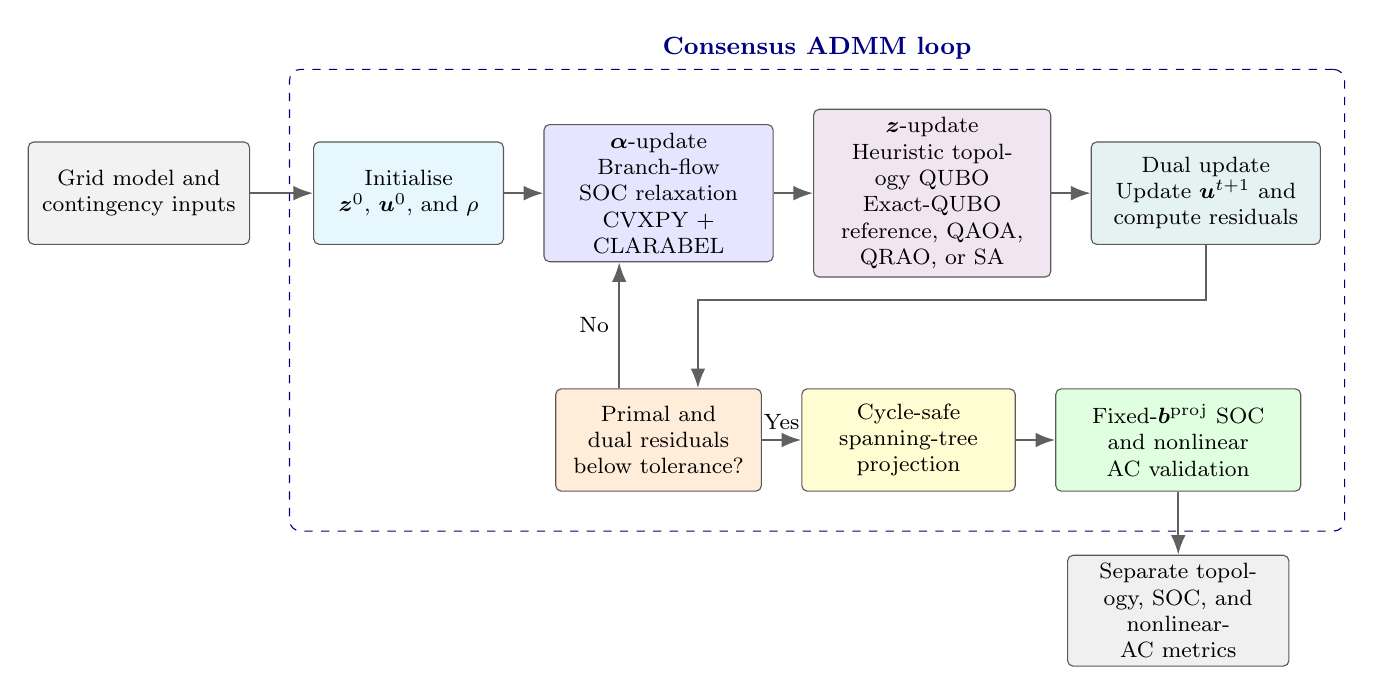
\begin{tikzpicture}[
  node distance=5mm and 5mm,
  font=\footnotesize,
  flow/.style={-{Latex[length=2.5mm]},thick,draw=gray!75!black},
  wfbox/.style={draw=gray!70!black,rounded corners=2pt,align=center,
    minimum height=13mm,inner sep=3pt},
  inputbox/.style={wfbox,fill=gray!10,text width=26mm},
  initbox/.style={wfbox,fill=cyan!10,text width=22mm},
  xbox/.style={wfbox,fill=blue!10,text width=27mm},
  zbox/.style={wfbox,fill=violet!10,text width=28mm},
  dualbox/.style={wfbox,fill=teal!10,text width=27mm},
  check box/.style={wfbox,fill=orange!15,text width=24mm},
  repairbox/.style={wfbox,fill=yellow!18,text width=25mm},
  validatebox/.style={wfbox,fill=green!12,text width=29mm},
  outputbox/.style={wfbox,fill=gray!12,text width=26mm}
]
  \node[inputbox] (input) {Grid model and\\contingency inputs};
  \node[initbox,right=8mm of input] (init) {Initialise\\$\boldsymbol z^0$, $\boldsymbol u^0$, and $\rho$};
  \node[xbox,right=of init] (xupdate) {$\boldsymbol\alpha$-update\\Branch-flow SOC relaxation\\CVXPY + CLARABEL};
  \node[zbox,right=of xupdate] (zupdate) {$\boldsymbol z$-update\\Heuristic topology QUBO\\Exact-QUBO reference, QAOA,\\QRAO, or SA};
  \node[dualbox,right=of zupdate] (dual) {Dual update\\Update $\boldsymbol u^{t+1}$ and compute residuals};

  \node[check box,below=16mm of xupdate] (check) {Primal and dual residuals below tolerance?};
  \node[repairbox,right=of check] (repair) {Cycle-safe spanning-tree projection};
  \node[validatebox,right=of repair] (validate) {Fixed-$\boldsymbol b^{\rm proj}$ SOC and nonlinear AC validation};
  \node[outputbox,below=8mm of validate] (output) {Separate topology, SOC, and\\nonlinear-AC metrics};

  \begin{scope}[on background layer]
    \node[draw=blue!45!black,dashed,rounded corners=4pt,
      fit=(init)(xupdate)(zupdate)(dual)(check),
      inner xsep=3mm,inner ysep=5mm,
      label={[font=\small\bfseries,text=blue!50!black]above:Consensus ADMM loop}] {};
  \end{scope}

  \draw[flow] (input) -- (init);
  \draw[flow] (init) -- (xupdate);
  \draw[flow] (xupdate) -- (zupdate);
  \draw[flow] (zupdate) -- (dual);
  \draw[flow] (dual.south) -- ++(0,-7mm) -|
    ([xshift=5mm]check.north);
  \draw[flow] ([xshift=-5mm]check.north) --
    node[left] {No} ([xshift=-5mm]xupdate.south);
  \draw[flow] (check) -- node[above] {Yes} (repair);
  \draw[flow] (repair) -- (validate);
  \draw[flow] (validate.south) -- (output.north);
\end{tikzpicture}
}
\caption{End-to-end workflow of the hybrid ADMM-QAOA pipeline. The
continuous $\boldsymbol\alpha$-update solves the branch-flow SOC relaxation,
while the discrete
$\boldsymbol z$-update solves the historical heuristic topology QUBO using an exact-QUBO,
quantum, or classical sub-solver. After convergence, the candidate is
projected onto a spanning tree by a cycle-safe Kruskal procedure and is
then checked by the fixed-$\boldsymbol b^{\rm proj}$ SOC model and
nonlinear AC recovery.}
\label{fig:pipeline-workflow}
\end{figure*}

\subsection{ADMM-inspired consensus iteration}
\label{sec:admm}
As a motivating consensus template, we use
$\boldsymbol z\in\{0,1\}^n$ for the binary QUBO copy,
$\boldsymbol\alpha\in[0,1]^n$ for its continuous SOC copy, and
$\boldsymbol u\in\mathbb R^n$ for the scaled dual variable. Physical
branch gates are obtained from either copy through
\eqref{eq:physical-gate-map}. The consensus constraint is
$\boldsymbol\alpha=\boldsymbol z$. Using iteration index $t$ (so it
cannot be confused with physical branch index $k$), the augmented
Lagrangian is
$\mathcal L_\rho(\boldsymbol\alpha,\boldsymbol z,\boldsymbol u)
=\Phi_{\mathrm{SOC}}(\boldsymbol\alpha)+g_Q(\boldsymbol z)
+(\rho/2)\|\boldsymbol\alpha-\boldsymbol z+\boldsymbol u\|_2^2$,
and the iteration is:

\begin{subequations}\label{eq:admm}
\begin{align}
\boldsymbol\alpha^{t+1} &:={}
\arg\min_{\boldsymbol\alpha\in[0,1]^n}
\Phi_{\mathrm{SOC}}(\boldsymbol\alpha)
+\tfrac{\rho}{2}
\|\boldsymbol\alpha-\boldsymbol z^t+\boldsymbol u^t\|_2^2,
\label{eq:admm-x}\\
\boldsymbol z^{t+1} &:={}
\arg\min_{\boldsymbol z\in\{0,1\}^n}g_Q(\boldsymbol z)
+\tfrac{\rho}{2}
\|\boldsymbol\alpha^{t+1}-\boldsymbol z+\boldsymbol u^t\|_2^2,
\label{eq:admm-z}\\
\boldsymbol u^{t+1} &:={}
\boldsymbol u^t+\boldsymbol\alpha^{t+1}-\boldsymbol z^{t+1}.
\label{eq:admm-y}
\end{align}
\end{subequations}

Here $\Phi_{\mathrm{SOC}}$ is the continuous SOC value function (losses plus
load-shed penalty) and $g_Q$ is the discrete heuristic topology prior. The
$\boldsymbol\alpha$-update is a convex SOCP solved by CLARABEL\@; the
$\boldsymbol u$-update is
an affine operation. In the released implementation $g_Q$ is a heuristic
bias, not an exact radiality or connectivity constraint. Consequently,
the released loop is classified as an ADMM-inspired consensus heuristic:
even with an exact QUBO subsolver it is not an exact decomposition of
the hard connected-radial problem, and QAOA introduces an additional
inexact subproblem solve. The final tree projection is post-processing
outside the iteration. We therefore report residuals and termination
conditions descriptively and make no generic ADMM convergence claim.
At iteration $t$, the complete binary objective in~\eqref{eq:admm-z}
is denoted $f_Q^{(t)}$; a QUBO minimum $f_Q^\star$ always refers to the
fully specified instance and iteration under discussion.

\subsection{Historical topology-coupled QUBO}
\label{sec:qubo}
A separable discrete prior $g_Q(\boldsymbol z)=0$ yields a
$\boldsymbol z$-update that decouples into $n$ independent binary
problems, each trivially solved by
$z_\ell=\operatorname{round}(\alpha_\ell+u_\ell)$; the quantum step then does
nothing that a one-line rounding could not do. The historical code
adds three topology-motivated terms. We retain them to preserve the
lineage of the frozen QAOA/QRAO results, but correct their mathematical
interpretation below.

\noindent\textbf{(1) Cardinality bias.}
With $K = |\mathcal{B}| - 1 - r_0$ the target number of closed
switches ($r_0$ is the rank of the always-closed sub-graph), the
term
$\lambda_{\text{card}}(\sum_\ell z_\ell-K)^2$
adds an all-pairs coupling of weight $2\lambda_{\text{card}}$ in
the QUBO's off-diagonal block. This is the correct switch count for a
tree only when the mandatory fixed sub-graph is a forest. If mandatory
fixed branches already contain a cycle, no setting of the remaining
switches can produce a spanning tree; a rank-based target does not
repair that infeasibility.

\medskip
\noindent\textbf{(2) Pairwise cycle bias.}
For each archived loop $C$ represented by variable positions, the term
$\lambda_{\text{cyc}}\sum_{\ell<m:\,\pi(\ell),\pi(m)\in C}
z_\ell z_m$ takes the value
$\lambda_{\text{cyc}}\binom{n_C}{2}$ when $n_C$ switches in $C$ are
closed. With a sufficiently large finite weight it penalises the
all-closed state of a two-switch parallel loop, but it does not make
that state infeasible. For $|C|>2$, it also penalises a valid acyclic
selection containing $|C|-1$ closed switches and is not equivalent to
the condition ``at least one cycle edge is open.''

\medskip
\noindent\textbf{(3) Pairwise anti-islanding bias.}
For each bus $i$ with no always-closed feed, we use the pairwise term
\begin{equation}
\begin{aligned}
g_i(\boldsymbol z)={}&-\lambda_{\text{iso}}
  \sum_{\ell:\,\pi(\ell)\in \operatorname{inc}(i)} z_\ell\\
&+\lambda_{\text{iso}}
  \sum_{\substack{\ell<m:\,\pi(\ell),\pi(m)\in
  \operatorname{inc}(i)}} z_\ell z_m.
\end{aligned}
\end{equation}
The exact isolated-bus indicator expands as
\begin{equation}
\prod_\ell(1-z_\ell)=1-\sum_\ell z_\ell
+\sum_{\ell<m}z_\ell z_m
-\sum_{\ell<m<q}z_\ell z_m z_q+\cdots .
\end{equation}
Consequently, the pairwise expression equals the product up to its
omitted constant for degree-one and degree-two buses. At higher degree the
discarded terms are essential, so this term is not a decomposition of
the isolated-bus indicator.

The total QUBO is

\begin{equation}\label{eq:qubo}
\begin{aligned}
\min_{\boldsymbol z\in\{0,1\}^n}\quad
&f_Q(\boldsymbol z)
=c_0+\boldsymbol q^\top\boldsymbol z
+\sum_{\ell<m}q_{\ell m}z_\ell z_m,\\
\boldsymbol q={}&\boldsymbol q^{\text{consensus}}
+\boldsymbol q^{\text{loss}}+\boldsymbol q^{\text{card}}
+\boldsymbol q^{\text{iso}},\\
q_{\ell m}={}&q_{\ell m}^{\text{card}}
+q_{\ell m}^{\text{cyc}}+q_{\ell m}^{\text{iso}}.
\end{aligned}
\end{equation}

The current implementation has $c_0=0$, but it is retained in the
notation because constants matter when converting to an Ising
Hamiltonian and expose why an objective ratio is offset-sensitive.
For completeness, the two separable linear components used by the code
at binary position $\ell$ are
\begin{align}
q_\ell^{\mathrm{consensus}}
&=\frac{\rho}{2}\!\left[1-2(\alpha_\ell+u_\ell)\right],\\
q_\ell^{\mathrm{loss}}
&=\eta\frac{r_{\pi(\ell)}}{\max_m r_{\pi(m)}+10^{-9}} .
\end{align}
The positive loss coefficient is a closing cost: under a fixed
cardinality it favors closing lower-resistance branches; without a
cardinality constraint it also biases switches toward open and must not
be interpreted as a physical loss calculation.

The audited union of nonzero off-diagonal pairs grows from
\MinQuboCouplings{} at $n=4$ to \MaxQuboCouplings{} at $n=12$
(Table~\ref{tab:qubo-growth}). The cardinality component already
occupies every pair, so the union is dense. The cycle component is
nevertheless nonzero at every size, and the anti-islanding component
is nonzero from $n=8$. Component counts overlap and therefore must not
be added to obtain the union count.

% Generated by artifact_pipeline.py; do not edit by hand.
\begin{table*}[t]
\centering
\caption{Audited nonzero off-diagonal QUBO pairs. Component counts can overlap; the union row counts nonzero pairs after all coefficients are summed.}
\label{tab:qubo-growth}
\small
\begin{tabular}{lccccc}
\toprule
$n$ & 4 & 6 & 8 & 10 & 12 \\
\midrule
Union after summation & 6 & 15 & 28 & 45 & 66 \\
Cardinality component & 6 & 15 & 28 & 45 & 66 \\
Cycle component & 2 & 3 & 6 & 7 & 8 \\
Anti-islanding component & 0 & 0 & 6 & 22 & 23 \\
\bottomrule
\end{tabular}
\end{table*}


The actual off-diagonal coefficients are nonuniform at every audited
size: they take values $6$ and $7.5$ at $n=4,6$, with additional
values $12$, $13.5$, and $19.5$ from $n=8$. Therefore the historical
QUBO is not the easy linear-plus-uniform-cardinality special case.
For completeness, the implementation includes the exact
$O(n\log n)$ sorting/prefix solver for that special case: for each
Hamming weight $m$, it selects the $m$ smallest linear coefficients
and compares the resulting $n+1$ energies. It agrees with exhaustive
enumeration at every audited size. The solver rejects the actual
nonuniform QUBO instead of being misreported as an applicable baseline.

\subsection{Flow-based connected-radial formulation and projection}
\label{sec:exact-radiality}
We use a single-commodity-flow formulation as the hard classical
reference. Orient every physical branch arbitrarily and let $h_k$ be
a signed artificial flow. Use the physical gate
$a_k(\boldsymbol z)$ from~\eqref{eq:physical-gate-map}. With the slack
bus denoted by $s$ and $M_h=|\mathcal B|-1$, impose
\begin{subequations}\label{eq:exact-radiality}
\begin{align}
\sum_{k\in\delta^+(i)}h_k-\sum_{k\in\delta^-(i)}h_k
&=\begin{cases}|\mathcal B|-1,&i=s,\\-1,&i\ne s,
\end{cases}\label{eq:tree-flow}\\
-M_h a_k(\boldsymbol z)\le h_k&\le M_h a_k(\boldsymbol z),
\qquad k\in\mathcal E,
\label{eq:tree-gate}\\
\sum_{\ell=0}^{n-1}z_\ell
&=|\mathcal B|-1-|\mathcal E^{\mathrm{mand}}|.
\label{eq:tree-cardinality}
\end{align}
\end{subequations}
The flow balances require every bus to be connected to the slack, and
the total of $|\mathcal B|-1$ closed branches then makes the connected
graph a tree. This equivalence assumes the mandatory fixed branches are
acyclic; the implementation explicitly declares the problem infeasible
otherwise. The reference is solved as a mixed-integer linear program
with SciPy/HiGHS. For these small instances we also enumerate every
bitstring and minimize the historical QUBO over radial states only.

The raw final ADMM bitstring $\boldsymbol b^{\rm raw}$ is handled by a
cycle-safe projection rather
than the earlier close-only connectivity repair. Kruskal's algorithm
first inserts every mandatory fixed branch, gives candidate-closed
switches priority, and then adds the lowest-impedance candidate-open
switches needed to connect the remaining components. Cycle-forming
candidate-closed switches are opened. The resulting operational
candidate is $\boldsymbol b^{\rm proj}$. The archived projection record lists
every opened and closed branch, the final closed-branch count,
connectivity, radiality, component count, and cycle rank.

\paragraph{ADMM iteration contract.}
We initialise $\boldsymbol z^0=\mathbf 1$ (all available decision
switches closed) and $\boldsymbol u^0=\boldsymbol 0$. At iteration $t$
the primal and dual residuals are, respectively,
$r_{\mathrm{pri}}^{t}=\|\boldsymbol\alpha^t-\boldsymbol z^t\|_2$ and
$r_{\mathrm{dual}}^{t}=\rho\|\boldsymbol z^t-
\boldsymbol z^{t-1}\|_2$. We terminate when both
fall below $10^{-2}$, or when 30 iterations have elapsed. The
raw final iterate is recorded as
$\boldsymbol b^{\rm raw}=\boldsymbol z^{t_{\rm stop}}$ and then projected
onto a spanning tree as described above. The distinct
$\boldsymbol b^{\rm proj}$ is solved with the corrected fixed-topology
SOC model, audited for cone, voltage-drop, thermal, and angle-recovery
residuals, and finally tested by nonlinear AC power flow. It is called
nonlinear-AC validated only if that check passes, and engineering-valid
only if the projected topology is also connected and radial.

\subsection{Quantum solvers}
\label{sec:quantum-solvers}
We compare four solver families for the QUBO: QAOA (noiseless and
noisy, with two depths), QRAO, an exact-QUBO reference solver, and the classical
SA metaheuristic. We provide short primers for the two quantum
solvers because the rest of the paper turns on their behaviour.

\paragraph{QAOA primer.}
QAOA~\cite{farhi2014qaoa} is a depth-$p$ variational algorithm for
Ising-type cost Hamiltonians. Applying
$z_\ell=(1-Z_\ell)/2$ to~\eqref{eq:qubo} gives the diagonal operator
\begin{subequations}\label{eq:qubo-ising}
\begin{align}
H_Q={}&\kappa I+\sum_\ell h_\ell Z_\ell
+\sum_{\ell<m}J_{\ell m}Z_\ell Z_m,\\
J_{\ell m}={}&\frac{q_{\ell m}}{4},\qquad
h_\ell=-\frac{q_\ell}{2}
-\frac14\sum_{m\ne\ell}q_{\min(\ell,m),\max(\ell,m)},\\
\kappa={}&c_0+\frac12\sum_\ell q_\ell
+\frac14\sum_{\ell<m}q_{\ell m}.
\end{align}
\end{subequations}
Thus every computational-basis state satisfies
$\langle\boldsymbol b|H_Q|\boldsymbol b\rangle=f_Q(\boldsymbol b)$,
including the additive constant. QAOA prepares
\begin{equation}
|\boldsymbol\gamma,\boldsymbol\beta\rangle
=\prod_{s=1}^{p}e^{-\mathrm i\beta_sH_M}
e^{-\mathrm i\gamma_sH_Q}|+\rangle^{\otimes n},
\qquad H_M=\sum_\ell X_\ell.
\end{equation}
The Qiskit \texttt{MinimumEigenOptimizer} path used here preserves the
QUBO's minimisation sense: COBYLA minimises
$\langle H_Q\rangle$, rather than maximising it. Sampling the resulting
state yields a returned bitstring $\boldsymbol b\in\{0,1\}^n$. For
$p=1$ the state is a 1-layer
alternating application of $H_Q$ and $H_M$; for $p=2$ we add a
second layer. We use COBYLA with $60$ iterations as the classical
optimizer in the ADMM demonstration; the retained scaling driver used
50 iterations, while the prospective protocol sets 100 iterations and
tolerance $10^{-4}$. The prospective noiseless runs use Qiskit's
shot-based reference \texttt{Sampler} V1 interface because Qiskit
Algorithms~0.3 and Qiskit Optimization~0.6.1 require its
\texttt{quasi\_dists} result contract; 4096 shots are used at each
objective evaluation. This pinned compatibility path is executable but
deprecated in Qiskit~1.2, and the warning is retained in the test log.
The legacy synthetic-noise runs attach a
depolarising noise model with per-qubit error $10^{-3}$ on
single-qubit gates and $2 \times 10^{-2}$ on two-qubit gates,
chosen as fixed simulation parameters rather than fitted calibration
values. Arrays returned by \texttt{MinimumEigenOptimizer} are in
QuadraticProgram variable order $[\pi(0),\ldots,\pi(n-1)]$; raw
measurement strings are stored separately and converted explicitly
before physical branches are addressed.

\paragraph{QRAO primer using the $(k,1,p)$-QRAC.}
QRAO~\cite{fuller2024qrao} packs $k$ binary variables per qubit
using a quantum random access code, a compression technique
borrowed from communication complexity. The idea is to encode
$\boldsymbol b\in\{0,1\}^k$ in a one-qubit state such that different
bits are associated with different Pauli observables. For the
$(3,1,p)$ code the implementation uses the ordered single-qubit
operators $X$, $Y$, and $Z$.

Qiskit's \texttt{QuantumRandomAccessEncoding} constructs the variable
grouping, Pauli assignment, and relaxed Hamiltonian subject to
\texttt{max\_vars\_per\_qubit=3}. The relaxed Hamiltonian generally
contains noncommuting single- and multi-qubit Pauli products. The
retained aggregate artifact archives only the reported qubit count,
not the variable-to-$(\text{qubit},\text{Pauli})$ assignment. The
prospective schema instead records \texttt{q2vars}, \texttt{var2op},
the relaxed-Hamiltonian offset, optimizer trace, and every retained
rounding sample. No causal packing claim is made from qubit count alone.

We approximate the relaxed Hamiltonian's minimum eigenstate with VQE,
a \texttt{RealAmplitudes(reps=1)} ansatz, and COBYLA. Qiskit's
\texttt{MagicRounding} then maps the relaxed result to candidate binary
bitstrings, which are rescored with the original $f_Q$. The retained
runs report a $1\times$ mapping, but without the archived assignment
that observation is not presented as a compression mechanism or
ablation result.
We use QRAO with \texttt{max\_vars\_per\_qubit=3} and a COBYLA optimiser
with 50 iterations in the retained scaling driver and 100 iterations in
the prospective protocol. For Qiskit Optimization 0.6.1, the prospective
wrapper evaluates MagicRounding measurement circuits in deterministic
batches of 256 rather than materialising all 4096 basis circuits at once
in the Python reference sampler.
The basis generator uses the trial seed and primitive batch $j$ uses
seed $\mathit{seed}+j$; these settings are archived with every run.
This is a memory-bounded execution of the same requested bases and shot
allocations, not a different rounding rule. Figure~\ref{fig:qrao-bloch} shows the
Bloch-sphere geometry of the three-bit QRAC encoding.

\begin{figure}[ht]
\centering
\resizebox{0.95\columnwidth}{!}{%
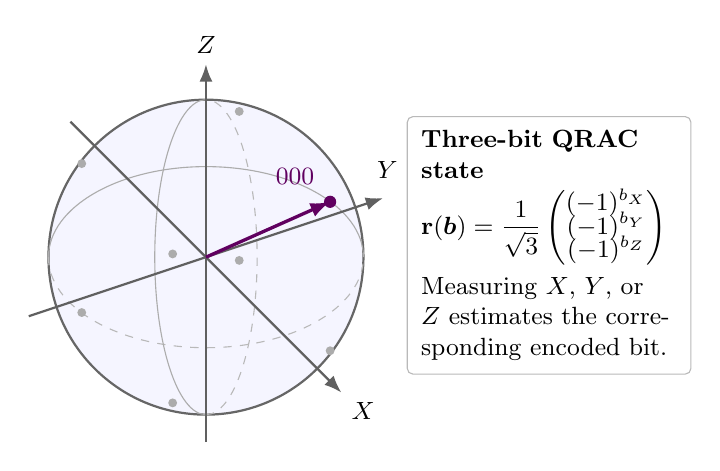
\begin{tikzpicture}[
  font=\small,
  axis/.style={-{Latex[length=2.2mm]},thick,draw=gray!75!black},
  state/.style={-{Latex[length=2.5mm]},very thick,draw=violet!75!black}
]
  \def\R{2.0}
  \fill[blue!4] (0,0) circle (\R);
  \draw[gray!80!black,thick] (0,0) circle (\R);

  % Equator and meridian: dashed arcs lie on the hidden hemisphere.
  \draw[gray!55,dashed] (-\R,0) arc[start angle=180,end angle=360,
    x radius=\R,y radius=1.15];
  \draw[gray!65] (\R,0) arc[start angle=0,end angle=180,
    x radius=\R,y radius=1.15];
  \draw[gray!55,dashed] (0,-\R) arc[start angle=-90,end angle=90,
    x radius=0.65,y radius=\R];
  \draw[gray!65] (0,\R) arc[start angle=90,end angle=270,
    x radius=0.65,y radius=\R];

  \draw[axis] (-1.72,1.72) -- (1.72,-1.72)
    node[below right] {$X$};
  \draw[axis] (-2.25,-0.75) -- (2.25,0.75);
  \node[anchor=south west] at (2.05,0.88) {$Y$};
  \draw[axis] (0,-2.35) -- (0,2.45) node[above] {$Z$};

  % Orthographic projection of the eight (3,1)-QRAC code states.
  % Camera azimuth = -30 degrees and elevation = 55 degrees.
  \foreach \sx/\sy/\sz in {
    1/1/1,1/1/-1,1/-1/1,1/-1/-1,
    -1/1/1,-1/1/-1,-1/-1/1,-1/-1/-1} {
    \pgfmathsetmacro{\px}{1.1547*(0.5*\sx+0.8660254*\sy)}
    \pgfmathsetmacro{\py}{1.1547*(-0.4967318*\sx
      +0.2867882*\sy+0.8191520*\sz)}
    \fill[gray!65] (\px,\py) circle (1.6pt);
  }

  \draw[state] (0,0) -- (1.577,0.703);
  \fill[violet!75!black] (1.577,0.703) circle (2.2pt);
  \node[anchor=south east,text=violet!75!black,font=\small\bfseries]
    at (1.50,0.80) {$000$};

  \node[anchor=west,align=left,draw=gray!55,rounded corners=2pt,
    fill=white,text width=3.25cm,inner sep=5pt] at (2.55,0.15) {
    \textbf{Three-bit QRAC state}\\[1mm]
    $\displaystyle
      \mathbf r(\boldsymbol b)=\frac{1}{\sqrt3}
      \begin{pmatrix}
        (-1)^{b_X}\\[-1mm]
        (-1)^{b_Y}\\[-1mm]
        (-1)^{b_Z}
      \end{pmatrix}$\\[1mm]
    Measuring $X$, $Y$, or $Z$ estimates the corresponding encoded bit.
  };
\end{tikzpicture}%
}
\caption{Bloch-sphere representation of the ideal three-variable
$(3,1,p)$ QRAC primitive permitted by the QRAO configuration. The eight
gray points correspond to the eight sign combinations of three encoded
bits; the highlighted $000$ state has equal positive components along
the Pauli $X$, $Y$, and $Z$ axes. This schematic is not evidence that
the retained runs packed three variables on each qubit.}
\label{fig:qrao-bloch}
\end{figure}

\paragraph{Simulated annealing (SA).}
A classical baseline: each iteration flips a uniformly random bit
with Metropolis acceptance and a geometric cooling schedule
$T_{t+1}=0.98T_t$ starting from $T_0=10$. The retained driver used
300 iterations; the prospective protocol uses 1000 iterations and
cooling factor $0.995$.

\paragraph{Exact QUBO reference.}
For the retained $n\le12$ instances, and likewise for the prospective
$n=13$ instance, we solve the QUBO exactly with the
\texttt{NumPyMinimumEigensolver}. It returns one
$\boldsymbol b_Q^\star\in\mathcal Z_Q^\star$ and the global QUBO value
$f_Q^\star$. This is an exact reference only for the historical
surrogate objective; it is not a reference for connectivity,
radiality, fixed-topology SOC loss, or nonlinear-AC validation.

\paragraph{Sorting/prefix reference.}
For the linear-plus-uniform-cardinality ablation, sorting the linear
coefficients and comparing all prefix lengths is exact. This baseline
is intentionally not applied to the historical QUBO, whose cycle and
anti-islanding terms make its pair coefficients nonuniform.

\paragraph{Hard-radial classical references.}
The single-commodity-flow MILP in~\eqref{eq:exact-radiality} provides a
polynomial-size exact spanning-tree formulation for a linear switch-cost
proxy. Independently, exhaustive enumeration minimizes the historical
quadratic objective over radial states only. Together these references
separate surrogate-objective optimality from topology feasibility.

\paragraph{Library implementation: \texttt{ADMMOptimizer} (3-ADMM-H).}
The repository contains a Qiskit~\texttt{ADMMOptimizer}
demonstration~\cite{qiskit_admm_optimizer} on a linearised surrogate.
Because the frozen artifact contains no numerical output for that
script, it is not included in the benchmark comparison.

\subsection{Hardware evidence scope}
\label{sec:hardware-contract}
Hardware execution is excluded from this submission because the
repository contains no validated repeated campaign. The executable
driver and offline validator remain as reproducibility infrastructure,
but no device-derived number enters a table, figure, or conclusion.
The repository documentation defines the required distinction among
sample expectation, modal sample, best observed sample, the complete
exact-QUBO minimizer set, and shot-level exact-optimum frequency. Any
future hardware claim must pass the archived evidence schema, retain raw
counts, job and calibration metadata, transpiled circuits, primitive
options, and same-instance topology/physics checks, and use repeated
matched jobs across calibration dates. A single baseline and
noise-management job would support descriptive reporting only.

% =====================================================================
\section{Benchmark Methodology}
\label{sec:benchmark}
% =====================================================================

\subsection{Retained artifact scope and archived variable ordering}
The frozen artifact used a historical \emph{base-case scaling sweep}:
the fault set was empty, $\mathcal F=\varnothing$. For each
$n\in\BenchmarkSizeSet$, only the first $n$ entries of the archived
switch order were binary variables and every later switch was forced
closed. The bus and branch data remained unchanged, but this rule creates
mandatory cycles for $n\in\RadialInfeasibleSizeSet$. The retained sweep
is therefore a surrogate-QUBO scaling artifact, not post-contingency
evidence and not a valid scaling sequence of the hard radial problem.

The historical QUBO parameters were
$\lambda_{\mathrm{card}}=3$,
$\lambda_{\mathrm{cyc}}=1.5$,
$\lambda_{\mathrm{iso}}=6$, and a loss-bias coefficient of $5$.
QAOA used $p\in\{1,2\}$, 1024 shots, COBYLA with at most 50 iterations,
and seeds $\{42,7,123\}$. The initial variational points were not
archived. SA used the same three seeds, 300 iterations, $T_0=10$, and
cooling factor $0.98$; the earlier statement of 400 iterations was
incorrect. Only one QRAO run per size survives in the aggregate artifact,
and its seed cannot be recovered. Consequently, the plotted standard
deviations are descriptive spread measures over three retained values,
not confidence intervals or evidence of a population distribution.

% Generated by study_protocol.py; do not edit by hand.
\begin{table*}[t]
\centering
\caption{Scope and predeclared regeneration protocol. The prospective row is a design specification, not a numerical result.}
\label{tab:study-protocol}
\small
\begin{tabularx}{\textwidth}{lXX}
\toprule
Item & Retained artifact & Prospective primary study \\
\midrule
Scenario & No forced outage (base case) & Hypothetical N$-1$ outage: Basantapur-Inaruwa ckt-A (branch 3) \\
Decision design & Prefix sizes $\{4,6,8,10,12\}$; omitted switches forced closed & Full remaining 13-switch decision set; no size sweep \\
Stochastic replication & Three QAOA/SA seeds; one retained QRAO run & 30 predeclared independent runs per stochastic method \\
QAOA & $p\in\{1,2\}$, 1024 shots, COBYLA 50 iterations; initial points not archived & $p\in\{1,2\}$, 4096 shots, COBYLA 100 iterations, tolerance $10^{-4}$; seeded initial points \\
SA & 300 iterations, $T_0=10$, cooling 0.98 & 1000 iterations, $T_0=10$, cooling 0.995 \\
Statistics & Descriptive only & Raw QUBO gaps $f_Q(\boldsymbol b)-f_Q^\star$; median/IQR; within-method percentile-bootstrap 95\% CI; Wilson 95\% CI for proportions \\
\bottomrule
\end{tabularx}
\end{table*}

% Generated by study_protocol.py; do not edit by hand.
\begin{table*}[t]
\centering
\caption{Archived binary-variable ordering. Zero-based vector positions $\ell$ map to physical branch indices $\pi(\ell)$.}
\label{tab:switch-order}
\small
\begin{tabular}{rrlrl}
\toprule
Legacy position & Branch & Physical element & Prospective position & Prospective status \\
\midrule
0 & 2 & Amarpur-Dhungesanghu 132 (tie+xfmr) & 0 & decision \\
1 & 3 & Basantapur-Inaruwa ckt-A & -- & forced open \\
2 & 4 & Basantapur-Inaruwa ckt-B & 1 & decision \\
3 & 5 & Baneshwar-Basantapur ckt-A & 2 & decision \\
4 & 6 & Baneshwar-Basantapur ckt-B & 3 & decision \\
5 & 7 & Tumlingtar-Baneshwar ckt-A & 4 & decision \\
6 & 8 & Tumlingtar-Baneshwar ckt-B & 5 & decision \\
7 & 9 & Dhungesanghu-Basantapur ckt-A & 6 & decision \\
8 & 10 & Dhungesanghu-Basantapur ckt-B & 7 & decision \\
9 & 12 & Inaruwa-Kusaha 132 & 8 & decision \\
10 & 13 & Duhabi-Kusaha 132 & 9 & decision \\
11 & 17 & Itahari-Dharan 132 & 10 & decision \\
12 & 18 & Amarpur-Phidim 132 & 11 & decision \\
13 & 20 & Godak-Damak 132 & 12 & decision \\
\bottomrule
\end{tabular}
\end{table*}


\subsection{Predeclared post-contingency protocol}
The separate regeneration protocol in
\code{results/study\_protocol.json} defines a hypothetical deterministic
N$-1$ outage of branch~3, Basantapur--Inaruwa circuit~A. This is a
reproducible scenario choice, not a claim that such a historical outage
occurred. The faulted branch is excluded from the bit vector, leaving the
13 variables and physical mapping in Table~\ref{tab:switch-order}. A
single-commodity-flow precheck confirms only that a spanning tree exists;
it is not evidence of SOC feasibility or nonlinear-AC validation. No size sweep is
used in the predeclared primary study, so every method is compared in the
same decision space.

Each stochastic method has 30 predeclared independent optimizer runs.
The same numeric seed labels are reused across methods only for
reproducibility; they do not create matched experimental units or
justify paired inference. QAOA and
QRAO use 4096 shots, COBYLA with 100 iterations and tolerance $10^{-4}$,
and seeded initial points drawn independently from
$\operatorname{Uniform}[-\pi,\pi)$ in the relevant ansatz parameter
order. QAOA uses $p\in\{1,2\}$; QRAO uses
\texttt{MagicRounding}. SA uses 1000 iterations, $T_0=10$, and cooling
factor $0.995$. Qiskit's algorithm-level random generator, variational
initial-point generator, and primitive sampling seed are all assigned the
same archived seed identifier.

For independent optimizer run $\nu=1,\ldots,R$, let
$\boldsymbol b^{(\nu)}$ be the returned variable-order bitstring. The
primary estimand is the offset-invariant QUBO gap
\begin{equation}
\Delta_Q^{(\nu)}=f_Q(\boldsymbol b^{(\nu)})-f_Q^\star,
\end{equation}
and the optimizer-run QUBO-minimum hit fraction is
\begin{equation}
\widehat h_{\mathrm{run}}^\star=\frac{1}{R}\sum_{\nu=1}^{R}
\mathbf 1\{\boldsymbol b^{(\nu)}\in\mathcal Z_Q^\star\}.
\end{equation}
This run-level statistic is distinct from a shot-level exact-optimum
frequency in a hardware sample.
Continuous quantities are summarized within each method by the
median, interquartile range, and a percentile-bootstrap 95\% confidence
interval using 10,000 resamples and fixed bootstrap seed 20260724.
Binary rates, including exact-QUBO hits, connected/radial outputs,
SOC recovery, and nonlinear-AC validation, use Wilson 95\% intervals.
Sensitivity analysis varies each QUBO weight
and ADMM $\rho$ one factor at a time by multipliers
$\{0.5,1,2\}$; those results are exploratory and support no causal claim.

ADMM uses constant $\rho=3$, all available switches initially closed,
$\boldsymbol u^0=\boldsymbol 0$, a 30-iteration limit, and primal and dual tolerances of
$10^{-2}$. Its $\boldsymbol z$-update uses
$\lambda_{\mathrm{card}}=0$,
$\lambda_{\mathrm{cyc}}=1.2$,
$\lambda_{\mathrm{iso}}=2.4$, and loss bias $0.9$. Every iteration must
archive both residuals, $\boldsymbol\alpha$, $\boldsymbol z$, losses,
shedding, termination reason, the raw final bitstring, the distinct
projected bitstring, and all projection actions.

The post-contingency solver output is archived in
\code{results/post\_contingency\_v1.json}; ADMM histories are archived in
\code{results/admm\_post\_contingency\_v1.json}. The generation pipeline
checks the protocol hash, trial counts, sensitivity artifact,
current-model validation, and statistics before writing the derived
tables, macros, figure, and SHA-256 manifest used below.

\subsection{Software and data}
All code, data, the network model, and the benchmark scripts are
released under the MIT licence in the project repository (see
\emph{Code availability}). The pinned environment uses Python~3.12.13,
CVXPY~1.5.3, CLARABEL~0.9.0, NetworkX~3.3, SciPy~1.14.1/HiGHS for the
radiality MILP, Qiskit~1.2.4, Qiskit Optimization~0.6.1, Qiskit
Algorithms~0.3.0, Qiskit Aer~0.15.1, and Qiskit IBM Runtime~0.30.0.
The complete operating-system, CPU, memory, package, Git, and timing
fingerprint is generated in \code{results/environment.json}.
Independent optimizer runs are isolated in separate processes. Up to
four run concurrently; every artifact records the actual worker count
and source commit. Deterministic QRAO circuit batching keeps this
execution within the documented 16-GB memory boundary.
Reported solver wall time covers the installed solver call, including
its variational optimization and sampling, but excludes process launch,
queueing, QUBO construction, topology projection, and physical
validation. No QPU-access time is reported.

\subsection{Reproducibility gates}
The legacy and post-contingency pipelines expose independent
\code{--check} modes. The latter refuses partial artifacts, mismatched
protocol hashes, missing or duplicate seeds, non-finite JSON values,
stale generated files, or manuscript inputs whose SHA-256 hashes differ
from the manifest. The primary, sensitivity, and ADMM artifacts share
the archived protocol hash, while \code{results/environment.json}
records the source commit and confirms that the source tree was clean at
generation time. The preserved
\code{results/benchmark\_legacy.json} contains historical non-standard
\code{Infinity} tokens and is provenance only; the migrated
\code{results/benchmark.json} is the strict authoritative legacy
artifact. Executable tests cover objective conventions, bit order,
QAOA/QRAO paths, process isolation, topology projection, and continuous
validation.

% =====================================================================
\section{Results}
\label{sec:results}
% =====================================================================

\subsection{Predeclared hypothetical post-contingency study}
The branch-3 scenario was executed exactly under the frozen protocol,
with \PostContingencyRunCount{} independent optimizer runs per method
(Table~\ref{tab:post-contingency-results}). QAOA at $p=1$ and $p=2$
share the lowest median offset-invariant QUBO gap,
\PostContingencyBestMedianGap{}; the generated deterministic tie break
labels \PostContingencyBestGapMethod{} as the first of these methods.
The corresponding percentile-bootstrap interval is
[\PostContingencyBestMedianGapCILower{},
\PostContingencyBestMedianGapCIUpper{}]. QAOA at $p=2$ has the largest
optimizer-run exact-QUBO hit fraction,
\PostContingencyBestHitFraction{}, but the overlapping intervals in
Table~\ref{tab:post-contingency-results} do not support a superiority
claim. The exact-QUBO reference has
\PostContingencyExactOptimumCount{} global minimizer.

% Generated by post_contingency_pipeline.py; do not edit by hand.
\begin{table*}[t]
\centering
\caption{Predeclared hypothetical N$-1$ post-contingency results. $\Delta_Q=f_Q(\boldsymbol{b})-f_Q^\star$. Gap intervals are within-method percentile-bootstrap 95\% intervals for the median; optimizer-run exact-QUBO hit intervals are Wilson 95\% intervals. Raw radiality is evaluated before projection; nonlinear AC validation is evaluated after the declared spanning-tree projection.}
\label{tab:post-contingency-results}
\small
\resizebox{\textwidth}{!}{%
\begin{tabular}{lrrrrrrrr}
\toprule
Method & $R$ & Median $\Delta_Q$ & 95\% CI & $\widehat h_{\rm run}^\star$ & 95\% CI & Median s & Raw radial & Projected nonlinear AC validated \\
\midrule
QAOA p1 noiseless & 30 & 0.500 & [0.250, 0.682] & 0.333 & [0.192, 0.512] & 7.586 & 0.000 & 1.000 \\
QAOA p2 noiseless & 30 & 0.500 & [0.000, 0.500] & 0.467 & [0.302, 0.639] & 12.078 & 0.000 & 1.000 \\
QRAO 3v & 30 & 0.682 & [0.250, 0.682] & 0.333 & [0.192, 0.512] & 396.378 & 0.000 & 1.000 \\
SA & 30 & 0.682 & [0.000, 0.682] & 0.400 & [0.246, 0.577] & 0.008 & 0.000 & 1.000 \\
\bottomrule
\end{tabular}
}
\end{table*}


Figure~\ref{fig:post-contingency-gaps} shows the complete seed-level gap
distributions. SA has millisecond-scale median wall time and the
quantum simulations provide no computational advantage. Across the
\PostContingencySensitivityVariantCount{} predeclared one-factor
variants, the QAOA-$p=1$ median gap ranges from
\PostContingencySensitivityMinMedianGap{} to
\PostContingencySensitivityMaxMedianGap{}
(Table~\ref{tab:post-contingency-sensitivity}). Each weight variant has
its own QUBO optimum, so this range is a tuning-sensitivity diagnostic,
not a cross-objective ranking. It nevertheless shows that the penalty
and optimizer settings are part of the reported result rather than
evidence of parameter robustness.

% Generated by post_contingency_pipeline.py; do not edit by hand.
\begin{table*}[t]
\centering
\caption{Predeclared one-factor-at-a-time QAOA-$p=1$ sensitivity audit. Each row contains 30 independent optimizer runs. Gap and hit statistics are defined relative to that row's own QUBO optimum; rows with different QUBO weights therefore diagnose tuning sensitivity but do not form a cross-objective performance ranking.}
\label{tab:post-contingency-sensitivity}
\small
\begin{tabular}{lrrrrrr}
\toprule
Varied factor & Setting & $R$ & Median $\Delta_Q$ & 95\% CI & $\widehat h_{\rm run}^\star$ & 95\% CI \\
\midrule
Primary & -- & 30 & 0.500 & [0.250, 0.682] & 0.333 & [0.192, 0.512] \\
$\lambda_{\mathrm{card}}$ & 1.5 & 30 & 0.500 & [0.000, 0.591] & 0.367 & [0.219, 0.545] \\
$\lambda_{\mathrm{card}}$ & 6 & 30 & 2.167 & [0.000, 2.667] & 0.400 & [0.246, 0.577] \\
$\lambda_{\mathrm{cyc}}$ & 0.75 & 30 & 0.083 & [0.042, 0.500] & 0.333 & [0.192, 0.512] \\
$\lambda_{\mathrm{cyc}}$ & 3 & 30 & 0.000 & [0.000, 0.000] & 0.867 & [0.703, 0.947] \\
$\lambda_{\mathrm{iso}}$ & 3 & 30 & 0.500 & [0.250, 0.682] & 0.333 & [0.192, 0.512] \\
$\lambda_{\mathrm{iso}}$ & 12 & 30 & 0.500 & [0.000, 0.682] & 0.400 & [0.246, 0.577] \\
Loss bias & 2.5 & 30 & 0.000 & [0.000, 0.000] & 0.900 & [0.744, 0.965] \\
Loss bias & 10 & 30 & 1.000 & [0.000, 1.000] & 0.433 & [0.274, 0.608] \\
COBYLA max iterations & 50 & 30 & 0.500 & [0.250, 0.682] & 0.333 & [0.192, 0.512] \\
COBYLA max iterations & 200 & 30 & 0.500 & [0.250, 0.682] & 0.333 & [0.192, 0.512] \\
\bottomrule
\end{tabular}
\end{table*}


\begin{figure}[t]
\centering
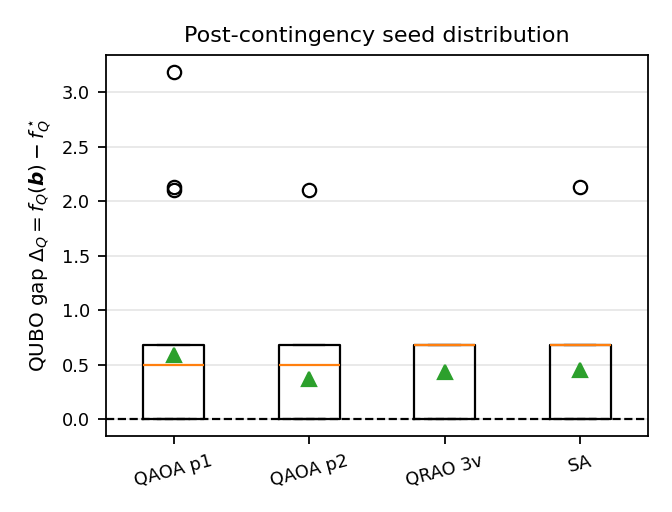
\includegraphics[width=\columnwidth]{koshi_admm_qaoa/figures/post_contingency_objective_gaps.png}
\caption{Seed-level offset-invariant QUBO gaps for the predeclared
hypothetical branch-3 contingency. Boxes show the interquartile range,
orange lines the median, green triangles the mean, and circles outliers.}
\label{fig:post-contingency-gaps}
\end{figure}

The raw and projected records have sharply different meanings
(Table~\ref{tab:post-contingency-validation}). No raw solver output is
connected or radial. The declared spanning-tree projection succeeds for
\PostContingencyBestGapProjectionPercent{}\% of the reported best-gap
runs, and \PostContingencyBestGapAcPercent{}\% of those projected
candidates pass the series-only nonlinear AC validation. The SOC
recovery rate is nevertheless
\PostContingencyBestGapSocPercent{}\% under the declared cone-slack
certificate. Thus the physical result is a property of the explicit
projection and subsequent validation, not of the raw QUBO output; the
nonlinear feasibility check is not an AC-OPF optimality certificate.

% Generated by post_contingency_pipeline.py; do not edit by hand.
\begin{table*}[t]
\centering
\caption{Topology and physical-validation audit for the prospective solver trials. Raw rates use solver outputs before repair. Projection and validation rates use the explicitly archived projected candidates. Voltage violation is the maximum excess beyond $[0.90,1.10]$ pu; thermal violation is the maximum utilization excess above 1. Loss is the median only among projected candidates passing the series-only nonlinear AC validation; a dash means no validated loss.}
\label{tab:post-contingency-validation}
\scriptsize
\resizebox{\textwidth}{!}{%
\begin{tabular}{lrrrrrrrrrrr}
\toprule
Method & $R$ & Raw C & Raw R & Projected & SOC recovered & AC validated & Max cone slack & Max angle residual & Max $|V|$ viol. & Max thermal viol. & Validated loss MW \\
\midrule
QAOA p1 noiseless & 30 & 0.000 & 0.000 & 1.000 & 0.000 & 1.000 & 1.04e-03 & 4.44e-16 & 1.02e-11 & 0.00e+00 & 4.101 \\
QAOA p2 noiseless & 30 & 0.000 & 0.000 & 1.000 & 0.000 & 1.000 & 1.04e-03 & 4.44e-16 & 1.02e-11 & 0.00e+00 & 4.101 \\
QRAO 3v & 30 & 0.000 & 0.000 & 1.000 & 0.000 & 1.000 & 1.04e-03 & 4.44e-16 & 1.02e-11 & 0.00e+00 & 4.101 \\
SA & 30 & 0.000 & 0.000 & 1.000 & 0.000 & 1.000 & 1.04e-03 & 4.44e-16 & 1.02e-11 & 0.00e+00 & 4.101 \\
\bottomrule
\end{tabular}
}
\end{table*}


\subsection{ADMM stopping audit}
% Generated by post_contingency_pipeline.py; do not edit by hand.
\begin{table*}[t]
\centering
\caption{Predeclared ADMM stopping audit. QAOA residuals are medians over independent optimizer runs.}
\label{tab:post-contingency-admm}
\small
\begin{tabular}{lrrrrl}
\toprule
Configuration & Runs & Iterations & Final primal & Final dual & Termination \\
\midrule
Exact-QUBO $\boldsymbol{z}$-update, $\rho=1.5$ & 1 & 30 & 2.650e+00 & 4.500e+00 & maximum\_iterations \\
Exact-QUBO $\boldsymbol{z}$-update, $\rho=3.0$ & 1 & 30 & 2.652e+00 & 9.000e+00 & maximum\_iterations \\
Exact-QUBO $\boldsymbol{z}$-update, $\rho=6.0$ & 1 & 30 & 2.653e+00 & 1.800e+01 & maximum\_iterations \\
QAOA $\boldsymbol{z}$-update, $\rho=3$ & 30 & -- & 2.219e+00 & 7.937e+00 & 0/30 converged \\
\bottomrule
\end{tabular}
\end{table*}


All exact-$\boldsymbol z$ penalty variants and all 30 QAOA-$\boldsymbol
z$ runs reach the predeclared 30-iteration cap. None satisfies both
residual tolerances, and none of the final QAOA--ADMM configurations
passes nonlinear AC validation. These data do not demonstrate ADMM
convergence or an engineering-feasible restoration; they delimit the
current implementation's failure under the frozen configuration.

\subsection{Coupled QUBO growth}
Figure~\ref{fig:qubo-growth} shows how the off-diagonal coupling count
in~\eqref{eq:qubo} grows with problem size. The union grows from
\MinQuboCouplings{} pairs at $n=4$ to \MaxQuboCouplings{} at $n=12$.
The cardinality component is dense, while the nonzero cycle and
anti-islanding counts overlap it. Density establishes coupling, but
does not by itself establish computational hardness.

\begin{figure}[ht]
\centering
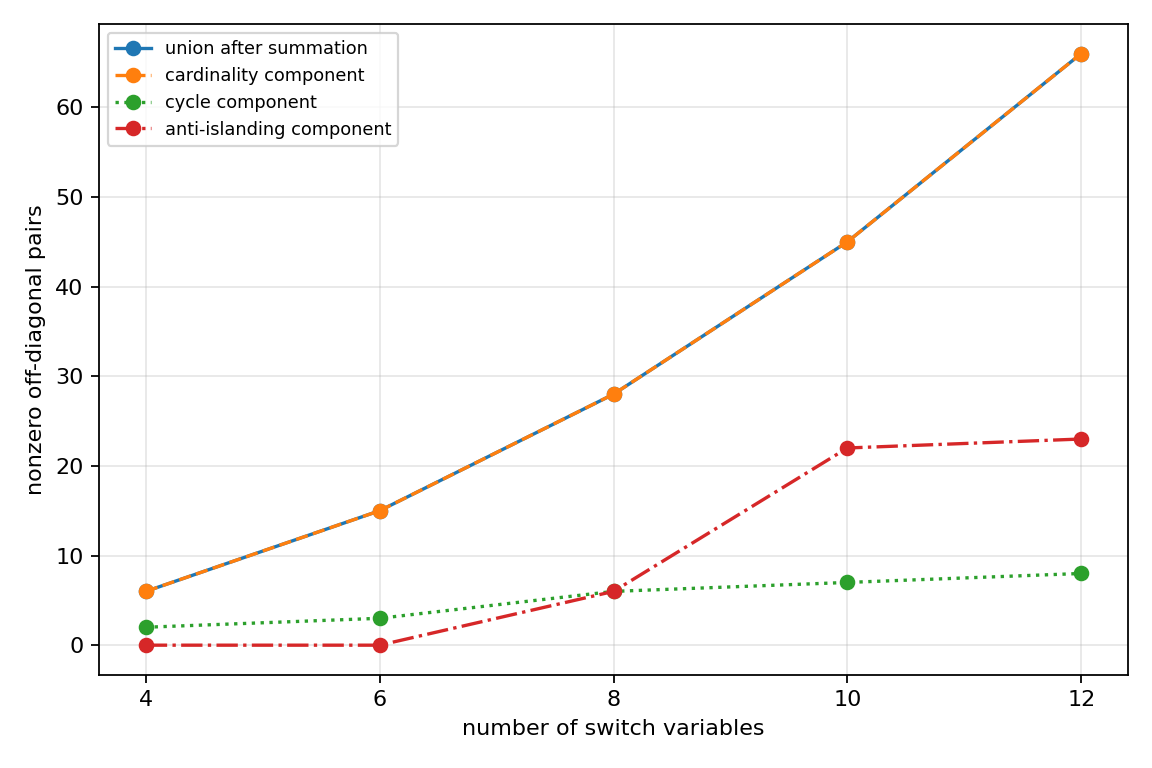
\includegraphics[width=\columnwidth]{koshi_admm_qaoa/figures/qubo_coupling_growth.png}
\caption{Audited nonzero off-diagonal QUBO pairs. Component curves can
overlap; the union curve counts nonzero pairs after coefficient
summation.}
\label{fig:qubo-growth}
\end{figure}

\subsection{Exhaustive radiality and surrogate-error audit}
% Generated by artifact_pipeline.py; do not edit by hand.
\begin{table*}[t]
\centering
\caption{Exhaustive topology audit of the historical scaling instances. FP counts radial states penalized by the pairwise cycle term; FN counts nonradial target-cardinality states receiving zero cycle penalty. The minimizer column is the number of radial members of $\mathcal Z_Q^\star$ divided by $|\mathcal Z_Q^\star|$. The final column is the best hard-radial QUBO value minus $f_Q^\star$; a dash means no radial state exists.}
\label{tab:radiality-audit}
\small
\begin{tabular}{rccccccc}
\toprule
$n$ & Fixed cycle rank & Tree feasible & Radial states & Cycle FP & Cycle FN & Radial/total $\mathcal Z_Q^\star$ & Hard-radial QUBO gap \\
\midrule
4 & 3 & no & 0 & 0 & 4 & 0/2 & -- \\
6 & 2 & no & 0 & 0 & 12 & 0/2 & -- \\
8 & 1 & no & 0 & 0 & 24 & 0/8 & -- \\
10 & 0 & yes & 32 & 12 & 45 & 0/3 & 2.290 \\
12 & 0 & yes & 64 & 24 & 20 & 0/3 & 1.478 \\
\bottomrule
\end{tabular}
\end{table*}


Table~\ref{tab:radiality-audit} exposes two independent failures of the
historical benchmark. First, the non-decision switches were forced
closed; at $n\in\RadialInfeasibleSizeSet$ those mandatory branches
already contain cycles, so the hard radial problem has no feasible
solution. Second, where radial states do exist ($n=10,12$), none of the
global historical-QUBO minimizers is radial. The pairwise cycle term
both penalises valid radial states (false positives) and assigns zero
cycle penalty to some nonradial target-cardinality states (false
negatives). These counts are exhaustive, not sampled. The actual QUBO
is nevertheless nonuniform at every size, so this failure is not
explained by the easy uniform-cardinality special case.

\subsection{QUBO objective ratio, optimizer-run exact-QUBO hit fraction,
and legacy SOC audit}
Figure~\ref{fig:approx-vs-size} separates the retained objective ratio
from the fraction of independent optimizer runs whose returned bitstring
attained $f_Q^\star$. The latter is not a probability estimated from QAOA or
QRAO samples. For noiseless QAOA at $p=1$, the $n=12$ values are
\QAOApOneTwelveRatio{} and \QAOApOneTwelveHitFraction{}, respectively.
QRAO returned a bitstring attaining $f_Q^\star$ in its single retained run at each
size, which is insufficient to estimate an optimizer-run hit fraction.

\begin{figure*}[ht]
\centering
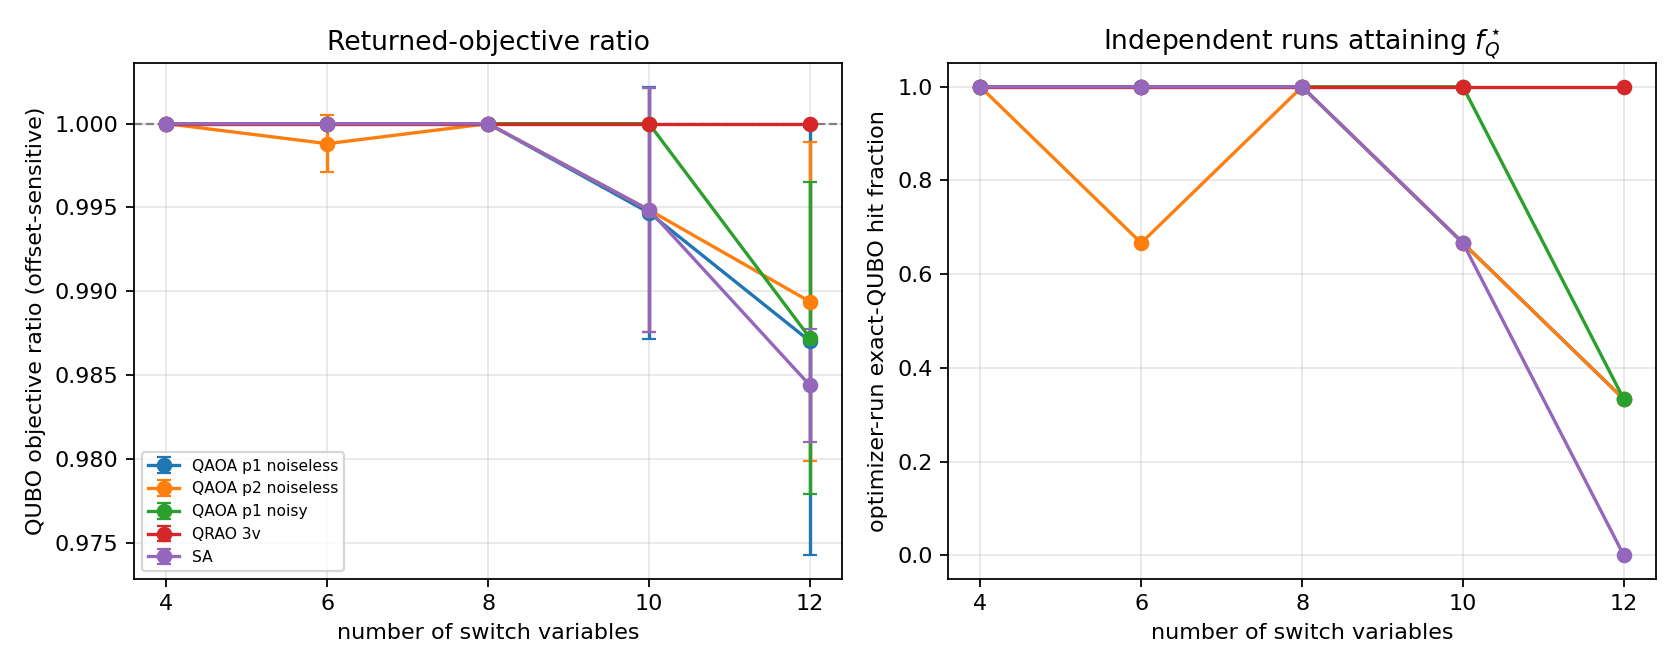
\includegraphics[width=0.95\textwidth]{koshi_admm_qaoa/figures/approx_vs_size.png}
\caption{Legacy offset-sensitive QUBO objective ratio (left) and the
optimizer-run exact-QUBO hit fraction $\widehat h_{\mathrm{run}}^\star$
(right).
QAOA and SA use three seeds; the legacy QRAO record contains one run per
size.}
\label{fig:approx-vs-size}
\end{figure*}

The legacy audit in Table~\ref{tab:legacy-soc-audit} retains SOC-loss,
connected, and feasibility fields that were computed before
continuous-model-v2. The historical exact-solver bitstrings were not
archived, so those fields cannot be tied to a recoverable returned
topology and are retained only to trace the original discrepancy.
Current exhaustive enumeration supplies the complete minimizer set of
the reconstructed QUBO, explicitly labelled as a reconstruction rather
than historical solver output. SA physics was not recorded. No current
SOC-loss, nonlinear-AC validation, or method-to-method physical
comparison is inferred from the legacy rows.

\subsection{Wall time and quantum-footprint comparison}
Figure~\ref{fig:walltime} plots the wall time of each solver against
problem size on a log scale. The classical exact-QUBO reference
solves the QUBO within \ExactQuboMaxTimeMs{}~ms at every $n$. QAOA $p=1$
noiseless takes \QAOApOneMinTime{}--\QAOApOneMaxTime{}~s; QAOA $p=1$
noisy reaches \NoisyQaoaMaxTime{}~s because of
noise-sampling overhead; \emph{no quantum speed-up is observed at this
scale}, which is the expected and honestly reported result.

\begin{figure}[ht]
\centering
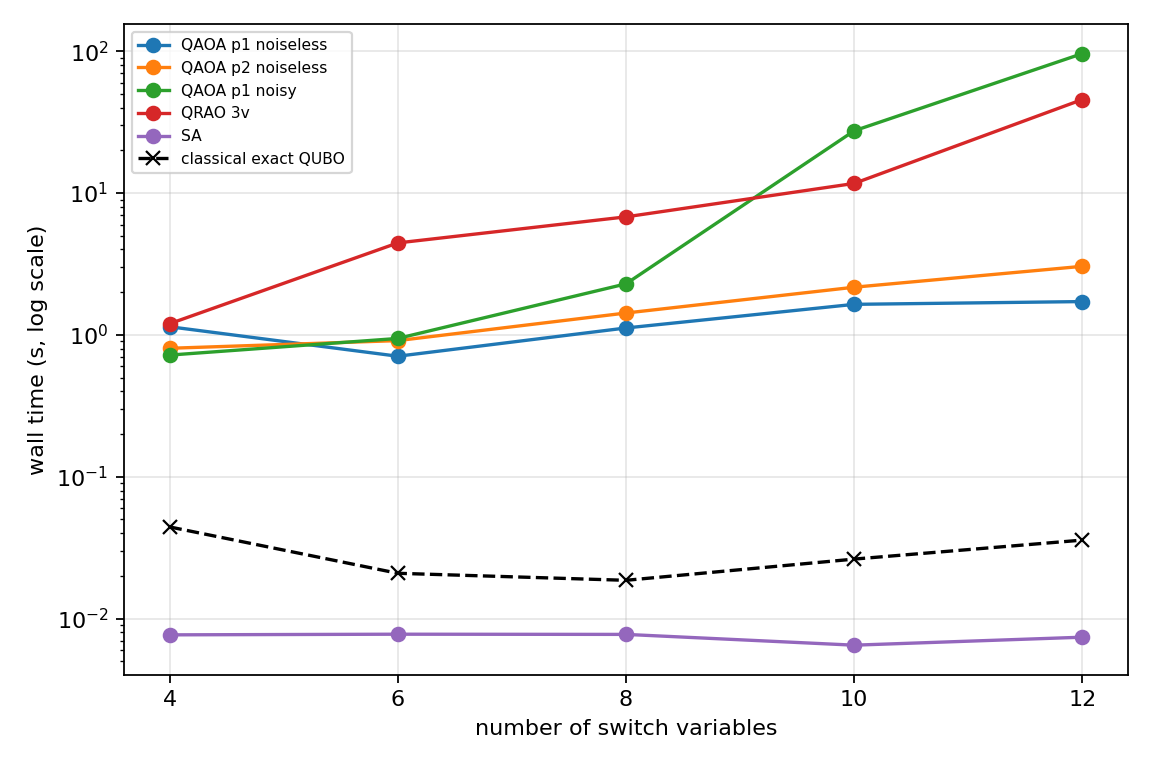
\includegraphics[width=\columnwidth]{koshi_admm_qaoa/figures/time_vs_size.png}
\caption{Mean wall time (s, log scale) versus problem size $n$ on a
single workstation. The classical exact-QUBO reference (black dashed) is
faster than every quantum variant at every $n$.}
\label{fig:walltime}
\end{figure}

Figure~\ref{fig:qubits} compares the qubit footprint of QAOA and QRAO
across the sweep.

\begin{figure}[ht]
\centering
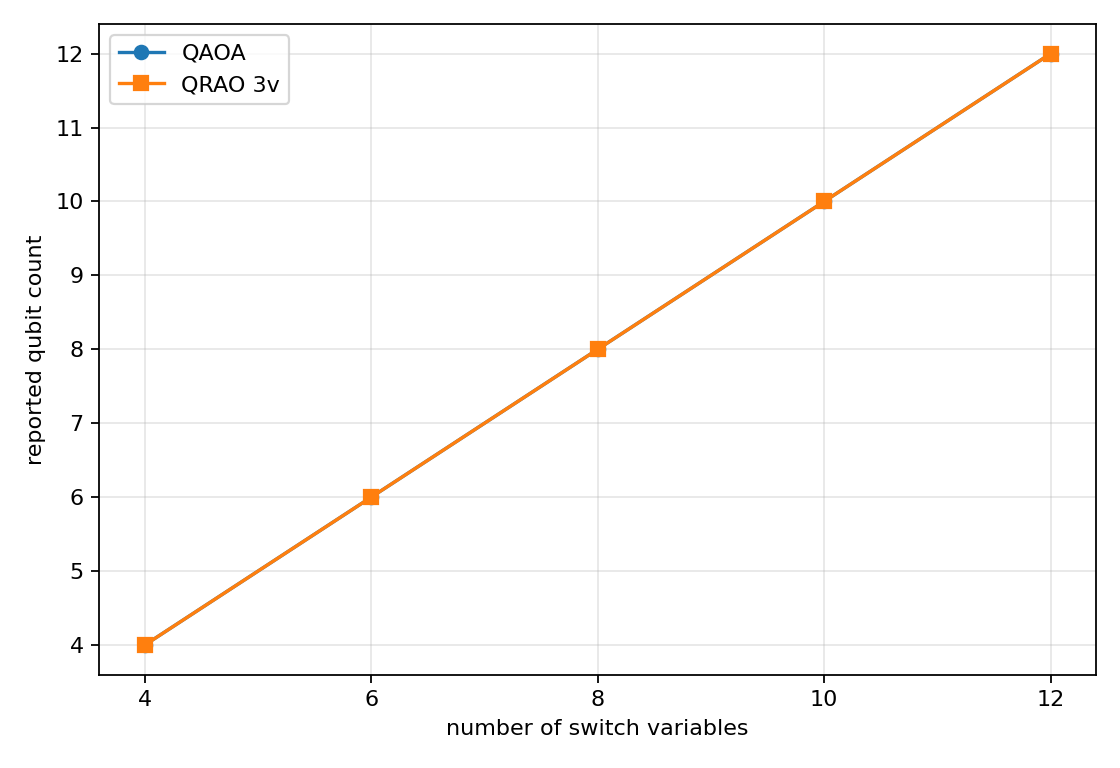
\includegraphics[width=\columnwidth]{koshi_admm_qaoa/figures/qubits_vs_size.png}
\caption{Reported QAOA and QRAO 3v qubit counts in the frozen artifact.
Both use one qubit per binary variable in the retained runs.}
\label{fig:qubits}
\end{figure}

\subsection{QRAO qubit footprint in the frozen record}
\label{sec:results-qrao}
The frozen record reports one QRAO run per size and one qubit per
binary variable, i.e.\ $\QraoReportedCompression$ compression
(Figure~\ref{fig:qubits}). The earlier manuscript attributed this
outcome to the cardinality term using a three-variant ablation, but no
machine-readable ablation output was released. That causal claim and
its table are therefore removed pending a regenerated, multi-seed
ablation artifact.

\subsection{Hardware evidence status}
\label{sec:results-hardware}
The repository did not release raw counts, exported job results,
backend and calibration metadata, or a machine-readable transpiled
circuit tied to the reported jobs. The previous hardware table,
figures, and causal noise/mitigation claims are therefore excluded
from the frozen result set. In particular, no retained value is relabelled
as a sampled-objective mean, modal sample, best observed QUBO sample, or global
QUBO minimum by inference.
The updated \code{phase3\_hardware.py} writes a timestamped schema-v2
evidence package containing raw counts, job metadata, backend/calibration
snapshots, archived variable order, trained parameters, QPY circuits, and
same-instance validation. The package must pass
\code{hardware\_evidence.py} before its generated tables can be placed at
the end of this subsection. No such validated package exists here.

\FloatBarrier

% =====================================================================
\section{Discussion}
\label{sec:discussion}
% =====================================================================

\subsection{Methodological lessons}
The case study surfaces three methodological lessons that are, in our
view, more general than the specific Eastern Nepal sub-system.

\paragraph{Lesson 1: Coupling is not constraint correctness.}
The cardinality term makes the union of off-diagonal pairs dense, but
the cycle and anti-islanding components are also nonzero and overlap
that union. A single total count cannot identify which physical
surrogates are active, and density alone establishes neither hardness
nor a correct radiality encoding. Component matrices, coefficient
ranges, and exhaustive false-positive/false-negative audits should
therefore be archived with every small benchmark instance.

\paragraph{Lesson 2: QUBO optimality is not engineering validity.}
The hard radial problem is structurally infeasible at $n=4,6,8$
because the supposedly fixed branches already contain cycles. At
$n=10,12$, radial states exist but no global historical-QUBO minimizer
is radial. The historical exact-solver bitstring is unavailable, so
the legacy connected/feasible field cannot support a claim about its
topology. Approximate QUBO ratios near one therefore cannot support
claims about connected, radial, SOC-recovered, or nonlinear-AC-validated
operation. Topology and continuous validation must be reported beside the
surrogate objective.

\paragraph{Lesson 3: Claim lineage is part of the experiment.}
The earlier paper mixed hard-coded prose, a one-panel figure, legacy
aggregate rows, and unarchived hardware/ADMM outputs. The revised
pipeline treats strict JSON as the source of truth and derives the CSV,
figures, macros, tables, and manifests from it. This permits negative
results---including zero raw-topology validity and failure of the ADMM
stopping test---to propagate into the manuscript without manual
reinterpretation. Unavailable results are marked NR or excluded rather
than copied from another method.

\subsection{Limitations and honest caveats}
The case study has the following honest limitations, which we list
explicitly rather than gloss over.

\begin{itemize}
\item The test system is not an as-operated network model. It combines
reported in-service assets, planned KC1 circuit~B, an under-construction
Amarpur--Dhungesanghu tie, and a hypothetical voltage interface.
Nodal MW/MVAr values, conductor impedances, ratings, taps, and several
segment lengths are assumptions. SCADA/EMS and utility planning data
would be required before operational conclusions.
\item The retained legacy continuous scores were generated by the
superseded continuous-model-v1. They are not results of the corrected
model and are not nonlinear AC power-flow or AC-OPF validation. The
separate hypothetical branch-3 study uses continuous-model-v2 but does
not retrofit physical validity onto the legacy scaling rows.
\item No contingency was applied in the retained legacy numerical
artifact. Those rows remain base-case surrogate-QUBO results. The new
branch-3 experiment is a deterministic hypothetical scenario, not an
observed outage or an operational restoration recommendation.
\item The historical QUBO topology terms are \emph{heuristic}; they
do not impose radiality or connectivity. The exhaustive audit and MILP
baseline are current, but the frozen quantum artifact did not retain
per-seed radiality flags or physics results.
\item The historical scaling sequence is not a valid hard-radial
scaling experiment at $n=4,6,8$. A future comparison must select
fixed-open/fixed-closed states that leave an acyclic mandatory subgraph,
or use the full switch set with a constraint-preserving encoding.
\item In the hypothetical contingency study, no raw stochastic-solver
candidate is connected or radial. All physically validated candidates
depend on the declared spanning-tree projection, and the SOC recovery
certificate rejects them at its numerical cone-slack threshold even
though the separate series-only nonlinear AC power flow converges. That
validation excludes shunts and phase-shifting transformers and is
neither full utility-model validation nor an AC-OPF certificate.
\item The ADMM residual test does not converge within 30 iterations for
any exact or QAOA-based run, and none of the QAOA--ADMM terminal
configurations passes nonlinear AC validation. The present results
therefore support no ADMM convergence or feasibility claim.
\item No quantum advantage is observed or claimed. The problem sizes
are too small, the depth too shallow, and the classical baselines
too strong. The contribution is the source-informed case study and the
auditable benchmark pipeline.
\item QRAO-ablation, Qiskit \texttt{ADMMOptimizer}, and hardware
conclusions remain excluded until their raw machine-readable evidence is
regenerated and archived. Every quantum result reported here is a local
simulation; no QPU performance claim is made.
\end{itemize}

% =====================================================================
\section{Conclusion}
\label{sec:conclusion}
% =====================================================================

We have presented an ADMM-inspired quantum-classical workflow for a
source-informed 16-bus Eastern Nepal test system and rebuilt the
numerical claim pipeline around a frozen artifact. The audit shows
that cycle and anti-islanding components were previously misreported as
empty, that the benchmark field named \texttt{success} was an
optimizer-run QUBO-minimum hit fraction rather than a sampled-bitstring
probability, and that the
historical pairwise terms do not encode radiality. Exhaustive enumeration
shows that the forced-closed scaling protocol makes the hard radial
problem infeasible at $n=4,6,8$ and that none of the historical QUBO
minimizers at $n=10,12$ is radial.
It also establishes that the retained driver supplied no forced-open
branch, so none of those numerical rows is a post-contingency result.
Continuous-model-v2 corrects shedding, thermal
limits, transformer taps, slack balance, and physical recovery.

The supported conclusions are therefore narrower: the retained QUBO
is nonuniform because cycle and anti-islanding coefficients modify the
dense cardinality component, but its topology terms are heuristic;
QRAO uses one qubit per variable in the retained runs; and the classical
exact-QUBO reference solver is faster than the quantum variants at these sizes.
The repository now includes a flow-based spanning-tree MILP, a
sorting/prefix baseline for the easy cardinality-only special case, and
a cycle-safe final projection with an explicit action log.

The separate predeclared hypothetical branch-3 study has now been
executed. QAOA at $p=1$ and $p=2$ share the lowest median QUBO gap,
\PostContingencyBestMedianGap{}, and QAOA $p=2$ has the largest
optimizer-run exact-QUBO hit fraction, but overlapping uncertainty
intervals and the much faster SA baseline support no quantum-advantage
or method-superiority claim. More decisively, no raw solver output is
connected or radial. The cycle-safe projection produces radial
candidates that pass the series-only nonlinear AC check, while none
passes the declared SOC-recovery certificate. All ADMM configurations
reach the iteration limit without satisfying both residual tolerances,
and the QAOA--ADMM terminal configurations fail nonlinear AC validation.
These outcomes make topology projection, validation lineage, and
negative stopping evidence central results rather than post-processing
details. Ablation and hardware conclusions remain deferred until
complete machine-readable evidence is available.

% =====================================================================
\section*{Code and data availability}
% =====================================================================
All code, data, and figures are released under the MIT licence at
\url{https://github.com/Zeeeepplin/koshi_admm_qaoa_v2}.
The \code{koshi\_admm\_qaoa} directory contains the network model, the
branch-flow SOC, the historical topology-coupled QUBO, the flow-based
radiality formulation and baselines in \code{radiality.py}, the ADMM
and QRAO solvers, the nonlinear AC recovery in \code{ac\_validation.py},
the frozen protocol in \code{results/study\_protocol.json}, the
statistical routines in \code{statistics\_report.py}, the benchmark
driver, and the Phase~3 hardware evidence-capture scripts. The
authoritative legacy benchmark file is
\code{results/benchmark.json}. The CSV, benchmark figures, numerical
macros, and appendix table are generated by
\code{artifact\_pipeline.py}; \code{results/artifact\_manifest.json}
records their SHA-256 hashes. The original aggregate JSON is retained
as \code{results/benchmark\_legacy.json} for provenance only. The
hypothetical branch-3 primary, sensitivity, and ADMM source artifacts
are respectively \code{results/post\_contingency\_v1.json},
\code{results/post\_contingency\_sensitivity\_v1.json}, and
\code{results/admm\_post\_contingency\_v1.json}.
\code{post\_contingency\_pipeline.py} validates them and records the
SHA-256 hashes of every post-contingency source and generated output in
\code{results/post\_contingency\_manifest.json}.

% =====================================================================
\appendix
% =====================================================================

\section{Legacy fixed-topology SOC-relaxation audit}
\label{app:legacy-soc-audit}
Table~\ref{tab:legacy-soc-audit} is generated directly from the frozen JSON
artifact. It reports only the legacy-v1 fixed-topology SOC information
that was retained; none of its loss values is eligible as a
continuous-model-v2 result. The QAOA rows describe the last seed scored by the
legacy driver, QRAO describes one run, and SA has no recorded physics
score. The row labelled ``Best connected SOC found (v1)'' is the
minimum recorded legacy fixed-topology SOC loss among connected
configurations evaluated by that enumeration; it is neither
$f_Q^\star$ nor a nonlinear AC optimum.

% Generated by artifact_pipeline.py; do not edit by hand.
\begin{table*}[t]
\centering
\caption{Legacy fixed-topology SOC audit retained for discrepancy tracing. All v1 losses and status codes predate continuous-model-v2 and are not eligible as current physical results. C denotes a recorded connected state; D denotes a disconnected state or a non-finite legacy SOC record whose cause was not separately archived; NR denotes not recorded.}
\label{tab:legacy-soc-audit}
\small
\begin{tabular}{lccccc}
\toprule
Method & $n=4$ & $n=6$ & $n=8$ & $n=10$ & $n=12$ \\
\midrule
One exact-QUBO minimizer & 5.83 (v1 C) & D-v1 & 5.92 (v1 C) & D-v1 & D-v1 \\
QAOA $p{=}1$ noiseless & 5.83 (v1 C) & D-v1 & 5.92 (v1 C) & D-v1 & D-v1 \\
QAOA $p{=}2$ noiseless & 5.83 (v1 C) & D-v1 & 5.92 (v1 C) & D-v1 & D-v1 \\
QAOA $p{=}1$ noisy & 5.83 (v1 C) & D-v1 & 5.92 (v1 C) & D-v1 & D-v1 \\
QRAO 3v & 5.83 (v1 C) & D-v1 & 5.92 (v1 C) & D-v1 & D-v1 \\
SA & NR & NR & NR & NR & NR \\
\midrule
Best connected SOC found (v1) & 5.73 & 5.73 & 5.73 & 5.73 & NR \\
\bottomrule
\end{tabular}
\end{table*}


% =====================================================================
\bibliography{references}
% =====================================================================

\end{document}
